\chapter{Quantum Monte Carlo}

\section{Modeling Diffusion}

Like any phenomena involving a density function, or distribution, Quantum Mechanics can be modeled by diffusion. In Quantum Mechanics, the distribution is given by $|\p|^2$, the Wave function squared. The diffusing elements of interest are the particles making up our system. The idea is to have an ensemble of \textit{Random Walkers} in which each walker represents a position is space (and time for time-dependent studies). Averaging values over the paths of the ensemble will yield average values corresponding to the probability distribution governing the movement of individual walkers. 

Such random movement is referred to as a \textit{Brownian motion}, named after the British Botanist R. Brown, originating from his experiments on plant pollen dispersed in water. \textit{Markov chains} are a subtype of Brownian motion, where a walkers next move is independent of previous moves. This is the stochastic process in which Quantum Monte Carlo is described.

The purpose of this section is to motivate the use of diffusion theory in Quantum Mechanics, and to derive the sampling rules needed in order to model Quantum Mechanical distributions by diffusion of random walkers correctly. I will be using natural units, that is $\hbar$, $m_e$, etc. are all set to unity, in order to simplify the expressions.

\subsection{Stating the Schrödinger Equation as a Diffusion Problem}
\label{sec:statingDiff}

Consider the time-dependent Schrödinger Equation for an abstract many-body wave function\footnote{See Section \ref{sec:manyBodyWFs} for details about many-body wave functions.} $\Phi(x, t)$ with an arbitrary energy shift $E'$

\begin{equation}
 -\frac{\partial \Phi(x, t)}{i\partial t} = (\OP{H} - E')\Phi(x, t).
\end{equation}

The formal solution given a time-independent Hamiltonian is given by separation of variables in $\Phi(x, t)$ (see ref. \cite{griffiths} for more details regarding assumptions etc.). This corresponds to using the standard time-evolution operator. Further expanding $\Phi(x, t=t_0)$ in the eigenstates of $\OP{H}$, $\Psi_k(x)$, yields the following solution

\begin{eqnarray}
 \Phi(x, t) &=& e^{-i(\OP{H} - E')(t-t_0)}\Phi(x, t=t_0) \label{eq:schrodGeneralSolution} \\
            &=& \sum_{k=0}^{\infty} C_k\Psi_k(x)e^{-i(E_k - E')(t-t_0)} \label{eq:realSchrod} \\
 C_k &=& \braket{\Psi_k(x)}{\Phi(x, t=0)} \nonumber
 \end{eqnarray}


The real form of this equation is obtained through a Wick rotation in time ($it \rightarrow \tau$), which basically means that the time-evolution operation is substituted by a \textit{projection operation}. To illustrate this, look at the solution of the real equation with $E'$ chosen to be the ground state energy of $\OP{H}$, and $t_0$ chosen to be zero

\begin{eqnarray}
 \Phi(x, \tau) &=& \sum_{k=0}^{\infty} C_k\Psi_k(x)e^{-(E_k - E_0)\tau} \label{eq:schrodGeneralSolution3}\\
                    &=& C_0\Psi_0(x) + \sum_{k=1}^{\infty} C_k\Psi_k(x)e^{-\delta E_k\tau}, \label{eq:schrodGeneralSolution2}
\end{eqnarray}

where $\delta E_k = E_k - E_0 > 0$ for $k \ge 1$. Observe that as $\tau$ increase, the excited states of $\OP{H}$ will be exponentially dampened, hence the name projection operation. Note however, that no real-time solutions can be achieved by solving this equation; only in the limit $\tau\rightarrow\infty$ will the solution match that of the Schrödinger Equation. 

The approach of Quantum Monte Carlo is to split the evolution of $\tau$ into small sequential steps $\delta\tau$, and use the latest calculated energy, the \textit{trial energy}, $E_T$, as an approximation to the ground state energy. The error introduced by this approximation will be discussed in Section~\ref{sec:DMC}. Either way, restating Eq.~(\ref{eq:schrodGeneralSolution3}) in terms of sequential steps yields

\begin{equation}
  \Phi(x, n\delta\tau) = \sum_{k=0}^{\infty} C_k\Psi_k(x)e^{-(E_k - E_T)n\delta\tau} \label{eq:genSolTimeSteps},
\end{equation}

which remains exact for an infinite amount of infinitely small time steps. In practice, a balance is sought between the \textit{number of cycles}, $n$, and the time step. This restatement might seem redundant, however, it is the key which opens up the possibility to model the solution by discretized diffusion of particles in Quantum Mechanical potentials. 

\subsection{Solving the Diffusion Problem}

In this chapter \textit{Dirac Notation} will be used. See Appendix \ref{app:Dirac} for an introduction.

Consider two sequential time steps $\tau$ and $\tau + \delta\tau$ in Eq.~(\ref{eq:genSolTimeSteps}). Without expanding the current state $\ket{\Phi(\tau)}$ like previously, we are left with an expression on the form

\begin{equation*}
 \ket{\Phi(\tau + \delta\tau)} = e^{-(\OP{H} - E_0)\delta\tau}\ket{\Phi(\tau)}.
\end{equation*}

Taking the inner product with $\bra{x}$ on both sides and inserting a complete set of states $\ket{y}$ on the left hand side yields

\begin{eqnarray*}
 \Phi(x, \tau + \delta\tau) &=& \int \bra{x}e^{-(\OP{H} - E_0)\delta\tau}\ket{y}\Phi(y, \tau)dy \\
			     &\equiv& \int G(x, y; \delta\tau)\Phi(y, \tau)dy
\end{eqnarray*}

where the \textit{Green's Function}, $G(x, y; \delta\tau)$ serves as a transition probability. This is the path integral formalism of Quantum Mechanics, where a final state is obtained by integrating through all possible paths of all the particles in the system, but I will not go into details about it here. More information about this can be found in ref. \cite{leinaas}. A more detailed derivation of the Green's Function are given in ref. \cite{abInitioMC}.

This is still not a practical way of solving the equations. In finding the Green's function we might as well find the solution directly. However, what we can do, is make the time steps very small and split the Hamiltonian into the kinetic, $\OP{T}$ and the potential part, $\OP{V}$:

\begin{eqnarray}
 \bra{x}e^{-(\OP{H} - E_0)\delta\tau}\ket{y} &=& \bra{x}e^{-(\OP{T} + \OP{V} - E_T)\delta\tau}\ket{y} \nonumber \\
                                             &=& \bra{x}e^{-\OP{T}\delta\tau}e^{-(\OP{V} - E_T)\delta\tau}\ket{y} + \frac{1}{2}[\OP{V}, \OP{T}]\delta\tau^2 + \mathcal{O}(\delta\tau^3) \nonumber \\
                                             &\simeq& \bra{x}e^{-\OP{T}\delta\tau}e^{-(\OP{V} - E_T)\delta\tau}\ket{y} 
\end{eqnarray}

The last step is known as the \textit{short time approximation}, that is, we split the Green's Function into two processes which are well known. The first which represents a diffusion process

\begin{equation}
\label{eq:GDiff}
 G_\mathrm{Diff} = e^{-\OP{T}\delta\tau}
\end{equation}

and the second which represents a branching process

\begin{equation}
 \label{eq:GB}
 G_\mathrm{B} = e^{-(\OP{V} - E_T)\delta\tau}
\end{equation}

Once a diffusion model is selected, for each cycle, the Green's functions are used to propagate the ensemble of walkers making up our distribution into the next time step. The final distributions of walkers will correspond to that of the direct solution of the Schrödinger Equation, given that the time step is sufficiently small, and we simulate long enough. These constraints will be covered in more detail later. 

Incorporating only the effect of Eq.(\ref{eq:GDiff}) results in a method called \textit{Variational Monte Carlo}. Including the branching term as well results in \textit{Diffusion Monte Carlo}. These methods will be discussed in sections \ref{sec:VMC} and \ref{sec:DMC}. In either of these methods, diffusion is the key process. In practice, we choose a diffusion model where closed form expressions for the Green's Functions exists. Two examples of this will be presented in the following sections.



\subsection{Isotropic Diffusion}

Isotropic diffusion is a process in which diffusing particles sees all possible directions as an equally probable path. Eq.~(\ref{Eq:diffusionSimple}) is an example of this. This is the simplest form of a diffusion equation, the case with a linear \textit{diffusion constant}, $D$, and no drift terms.

\begin{equation}
 \label{Eq:diffusionSimple}
 \frac{\partial P(\vec r, t)}{\partial t} = D\nabla^2 P(\vec r, t) 
\end{equation}

In the Quantum Monte Carlo case, the value of the diffusion constant is $D=\frac{1}{2}$, that is, the term scaling the Laplacian in the Schrödinger Equation. The closed form expression for the Green's function is a Gaussian distribution with variance $2D\delta t$ \cite{abInitioMC}

\begin{equation}
\label{eq:GF_iso}
 G_{\mathrm{Diff}}^{\mathrm{ISO}}(i\,\rightarrow j) \propto e^{-(x_i-x_j)^2/4D\delta\tau}  .
\end{equation}

These equations describe the diffusion process theoretically, however, in order to achieve specific sampling rules for our walkers, we need a connection between the time-dependence of the total distribution and the time-dependence of an individual walker's components in configuration space. This connection is given in terms of a stochastic differential equation called \textit{The Langevin Equation}.

\subsubsection{The Langevin Equation for Isotropic Diffusion}

The Langevin Equation is a stochastic differential equation used in physics to relate the time dependence of a distribution to the time-dependence of the degrees of freedom in the system. For the simple isotropic diffusion described previously, solving the Langevin equation using a Forward Euler approximation for the time derivative results in the following relation:

\begin{eqnarray}
\label{eq:langevinSolSimple}
 x_{i+1} = x_i + \xi, \qquad\qquad \mathrm{Var}(\xi) &=& 2D\delta t, \\
			     \langle\xi\rangle &=& x_i, \nonumber 
\end{eqnarray}

where $\xi$ is a normal distributed number whose variance match that of the Green's function in Eq.~(\ref{eq:GF_iso}). This relation is in agreement with the isotropy of Eq.~(\ref{Eq:diffusionSimple}) in the sense that the displacement is symmetric around the current position.


\subsection{Anisotropic Diffusion: Fokker-Planck}
\label{sec:anisFokker}

Anisotropic diffusion, in contrast to isotropic diffusion, does not count all directions as equally probable. An example of this is diffusion according to the \textit{Fokker-Planck Equation}, that is, diffusion with a drift term, $\vec F(\vec r, t)$, responsible for pushing the walkers in the direction of configurations with higher probabilities.

\begin{equation}
 \label{Eq:fokkerPlanck}
 \frac{\partial P(\vec r, t)}{\partial t} = D\nabla\cdot\Big[\Big(\nabla - \vec F(\vec r, t)\Big) P(\vec r, t)\Big] 
\end{equation}

The remarkable thing is that simple isotropic diffusion processes obey this relation \cite{abInitioMC}. This means that Quantum Mechanical distributions can be modeled by the Fokker-Planck Equation, leading to a more optimized way of sampling in practical situations. 

In Quantum Monte Carlo we want convergence to a stationary state. We can use this criteria to deduce expression for the drift term given our Quantum Mechanical distribution. A stationary state is obtained when the left hand side of Eq.~(\ref{Eq:fokkerPlanck}) is zero:

\begin{equation*}
 \nabla^2 P(\vec r, t) = P(\vec r, t)\nabla\cdot\vec F(\vec r, t) + \vec F(\vec r, t) \cdot \nabla P(\vec r, t)
\end{equation*}

The next thing we want to achieve is cancellation in the rest of the terms. In order to obtain a Laplacian term on the right hand side to potentially cancel out the one on the left, the drift term needs to be on the form $F(\vec r, t) = g(\vec r, t)\nabla P(\vec r, t)$. Inserting this yields

\begin{equation*}
  \nabla^2 P(\vec r, t) = P(\vec r, t)\frac{\partial g(\vec r, t)}{\partial P(\vec r, t)}\Big|\nabla P(\vec r, t)\Big|^2
  + P(\vec r, t)g(\vec r, t)\nabla^2 P(\vec r, t) + g(\vec r, t) \Big|\nabla P(\vec r, t)\Big|^2.
\end{equation*}

Looking at the factors in front of the Laplacian suggests using $g(\vec r, t) = 1/P(\vec r, t)$. A quick check reveals that this also cancels out the gradient terms, and the resulting expression for the drift term becomes

\begin{eqnarray}
 \vec F(\vec r, t) &=& \frac{1}{P(\vec r, t)}\nabla P(\vec r, t) \nonumber \\
                   &=& \frac{2}{|\psi(\vec r, t)|}\nabla |\psi(\vec r, t)|
\end{eqnarray}

In Quantum Monte Carlo, the drift term is called \textit{The Quantum Force}, since it is responsible for pushing the walkers into regions of higher probabilities, analogous to a force in Newtonian mechanics.

Another strength of the Fokker-Planck equation is that even though the equation itself is more complicated, it's Green's function still has a closed form solution. This means that we can evaluate it efficiently. If this was not the case, the practical value would be reduced dramatically. The reason for this will become clear in Section \ref{sec:MetroMain}. As expected, it is no longer symmetric 

\begin{equation}
\label{eq:GF_FP}
 G_\mathrm{Diff}^\mathrm{FP}(i\,\rightarrow j) \propto e^{-(x_i-x_j - D\delta\tau F(x_i))^2/4D\delta\tau}.
\end{equation}


\subsubsection{The Langevin Equation for the Fokker-Planck Equation}

The Langevin equation in the case of a Fokker-Planck Equation has the following form

\begin{equation}
 \frac{\partial x_i}{\partial t} = D F(x_i) + \eta,
\end{equation}

where $\eta$ is a so-called \textit{noise term} from stochastic processes. Solving this using the same method as for the isotropic case yields the following sampling rules

\begin{equation}
 \label{eq:langevinSolFP}
 x_{i+1} = x_i + \xi + DF(x_i)\delta t,
\end{equation}

where $\xi$ is the same as for the isotropic case. We observe that if the drift term is set to zero, we are back in the isotropic case, just as required. For more details regarding the Fokker-Planck Equation and the Langevin equation, see ref. \cite{Gardiner:2004bk}, \cite{risken1989fpe} and \cite{langevin}.


\subsubsection{Importance sampling}

It can be shown, see e.g. Ref. \cite{abInitioMC}, that the relationship between the isotropic and anisotropic diffusion model of the complex time Schrödinger Equation is simply that we have multiplied the Schrödinger equation by a known function $\Psi_T(x)$, i.e.

\begin{eqnarray}
 \frac{\partial }{\partial \tau}\Phi(x, \tau) &\quad\Longrightarrow\quad& \frac{\partial }{\partial \tau}\left(\Phi_T(x)\Phi(x, \tau)\right) \\
 G_\mathrm{Diff}^\mathrm{ISO}  &\quad\Longrightarrow\quad&  G_\mathrm{Diff}^\mathrm{FP}
\end{eqnarray}

Just as in traditional importance sampled Monte-Carlo integrals, optimized sampling is obtained by switching distributions into one which exploits known information about the problem at hand. In case of standard Monte-Carlo integration, we switch sampling distribution to one which are similar to the original integrand, i.e. smoothing out the sampled function, where as for Quantum Monte-Carlo, we use a function which is constructed with the sole purpose of imitating the exact ground state to suggest moves more efficiently. It is therefore reasonable to call the use of Fokker-Planck diffusion \textit{Importance sampled Quantum Monte-Carlo}.

This new function, $\Psi_T(x)$, is referred to as a \textit{trial wave function}, and will be discussed in more detail in Section \ref{sec:trialWF}.


\section{Diffusive Equilibrium Constraints}

Upon convergence of a Markov process, the system at hand will reach its most likely state. This is exactly the behaviour of a real system of diffusing particles described by statistical mechanics: It will \textit{thermalize}, that is, be in its most likely state given a surrounding temperature. Markov processes are hence beloved by physicists; they are simple, yet realistic. 

Once thermalization is reached, average values may be sampled. However, simply spawning a Markov process and waiting for thermalization is an inefficient and unpractical scenario. This may take forever, and it may not; either way its not optimal. We can introduce rules of acceptance and rejection of transitions purposed by following the solutions of the Langevin Equation (Eq.~(\ref{eq:langevinSolSimple}) and Eq.~(\ref{eq:langevinSolFP})), but not without constraints. If any of the following conditions break, we have no guarantee that the system will thermalize properly:

\subsection{Detailed Balance} 

For Markov processes, detailed balance is achieved by demanding a \textit{Reversible} Markov process. This boils down to a statistical requirement stating that 

\begin{equation}
 \label{eq:DetailedBalance}
 P_iW(i\,\rightarrow\,j) = P_jW(j\,\rightarrow\,i),
\end{equation}

where $P_i$ is the probability density in configuration $i$, and $W(i\,\rightarrow\,j)$ is the transition probability between states $i$ and $j$. 

\subsection{Ergodicity}

Another requirement is that the sampling must be ergodic, that is, the Markov chain (or simpler: The walker) needs to be able to be able to reach any configuration state in the space spanned by the distribution function. It is tempting to define a brute force acceptance rule where only steps resulting in a higher overall probability is accepted, however, this limits the path of the walker, and hence breaks the ergodicity requirement.

\section{The Metropolis Algorithm}
\label{sec:MetroMain}

The Metropolis Algorithm is a simple set of acceptance/rejection rules used in order to make the thermalization more effective. I will not go into details about transport theory in this section, but rather start the derivation from the criteria of detailed balance, Eq.~(\ref{eq:DetailedBalance}), modeling the transition probability as two-part: $g(i\,\rightarrow\,j)$, the probability of selecting configuration $j$ given configuration $i$, times a probability of accepting the selected move, $A(i\,\rightarrow\,j)$:

\begin{eqnarray}
 \label{eq:metro1}
 P_iW(i\,\rightarrow\,j) &=& P_jW(j\,\rightarrow\,i) \nonumber \\
 P_ig(i\,\rightarrow\,j)A(i\,\rightarrow\,j) &=& P_jg(j\,\rightarrow\,i)A(j\,\rightarrow\,i)
\end{eqnarray}

Inserting the probability distribution as the Wave function squared, and the selection probability as our Green's function, then gives us a simple expression:

\begin{eqnarray}
  \label{eq:metro2}
  |\psi_i|^2G(i\,\rightarrow\,j)A(i\,\rightarrow\,j) &=& |\psi_j|^2G(j\,\rightarrow\,i)A(j\,\rightarrow\,i) \nonumber \\
  \frac{A(j\,\rightarrow\,i)}{A(i\,\rightarrow\,j)} &=& \frac{G(i\,\rightarrow j)}{G(j\,\rightarrow i)}\frac{|\psi_i|^2}{|\psi_j|^2} \equiv R_G(j\,\rightarrow\,i)R_\psi(j\,\rightarrow\,i)^2
\end{eqnarray}

Assume now that configuration $i$ has a higher overall probability than configuration $j$, that is, $A(i\,\rightarrow\,j) = 1$. A more effective thermalization is obtained by accepting all these moves. What saves us from breaking the criteria of ergodicity is the fact that we do not reject the move otherwise. Instead, we insert $A(i\,\rightarrow\,j) = 1$ into Eq.~(\ref{eq:metro2}), and thus ensuring detailed balance as well as ergodicity. This yields

\begin{equation*}
 A(j\,\rightarrow\,i) = R_G(j\,\rightarrow\,i)R_\psi(j\,\rightarrow\,i)^2
\end{equation*}


Concatenating both scenarios yields the following acceptance/rejection rules:

\begin{equation}
\label{eq:MetroGeneralGreen}
 A(i\,\rightarrow\,j) = \left\{\begin{array}{ccc}
R_G(i\,\rightarrow\,j)R_\psi(i\,\rightarrow\,j)^2 & & R_G(i\,\rightarrow\,j)R_\psi(i\,\rightarrow\,j)^2 < 1\\
1  & & \mathrm{else}  \end{array}\right. 
\end{equation}

Or more simplistic:

\begin{equation}
  A(i\,\rightarrow\,j) = \min\{R_G(i\,\rightarrow\,j)R_\psi(i\,\rightarrow\,j)^2, \,1\}
\end{equation}


For the isotropic case, we have a cancellation of the Greens function due to symmetry, $R_G(i\,\rightarrow\,j) = 1$, leaving us with the standard Metropolis algorithm:

\begin{equation}
\label{eq:Metropolis_standard}
 A(i\,\rightarrow\,j) = \min\{R_\psi(i\,\rightarrow\,j)^2, \,1\}
\end{equation}

If we on the other hand use the Fokker-Planck equation, we will not get a cancellation. Inserting Eq.~(\ref{eq:GF_FP}) into Eq.~(\ref{eq:MetroGeneralGreen}) results in the \textit{Metropolis Hastings algorithm}. The ratio of Green's function can be evaluated efficiently by simply subtracting the exponents of the exponentials

\begin{eqnarray}
 R_G^\mathrm{FP}(i\,\rightarrow\,j) &=&G_\mathrm{Diff}^\mathrm{FP}(j\,\rightarrow i)/G_\mathrm{Diff}^\mathrm{FP}(i\,\rightarrow j) \nonumber \\
                                    &=& \exp{\Big[\frac{1}{2}\big(F(x_j) + F(x_i)\big)\big(\frac{1}{2}D\delta t(F(x_j) - F(x_i)) + x_i - x_i\big)\Big]}
\end{eqnarray}

\begin{equation}
\label{eq:MetropolisHastings}
 A(i\,\rightarrow\,j) = \min\{R_G^\mathrm{FP}(i\,\rightarrow\,j)R_\psi(i\,\rightarrow\,j)^2, \,1\}
\end{equation}

Derived from detailed balance, the Metroplis Algorithm is as a must-have when it comes to Markov Chain Monte Carlo. Besides Quantum Monte Carlo, we have methods such as the \textit{Ising Model} which greatly benefit from these rules \cite{morten}.

A chart flow describing the implementation of the Metropolis algorithm and the diffusion process in general is given in Fig. \ref{fig:diffFlowChart}.

\begin{figure}
\label{fig:diffFlowChart}
 \begin{center}
  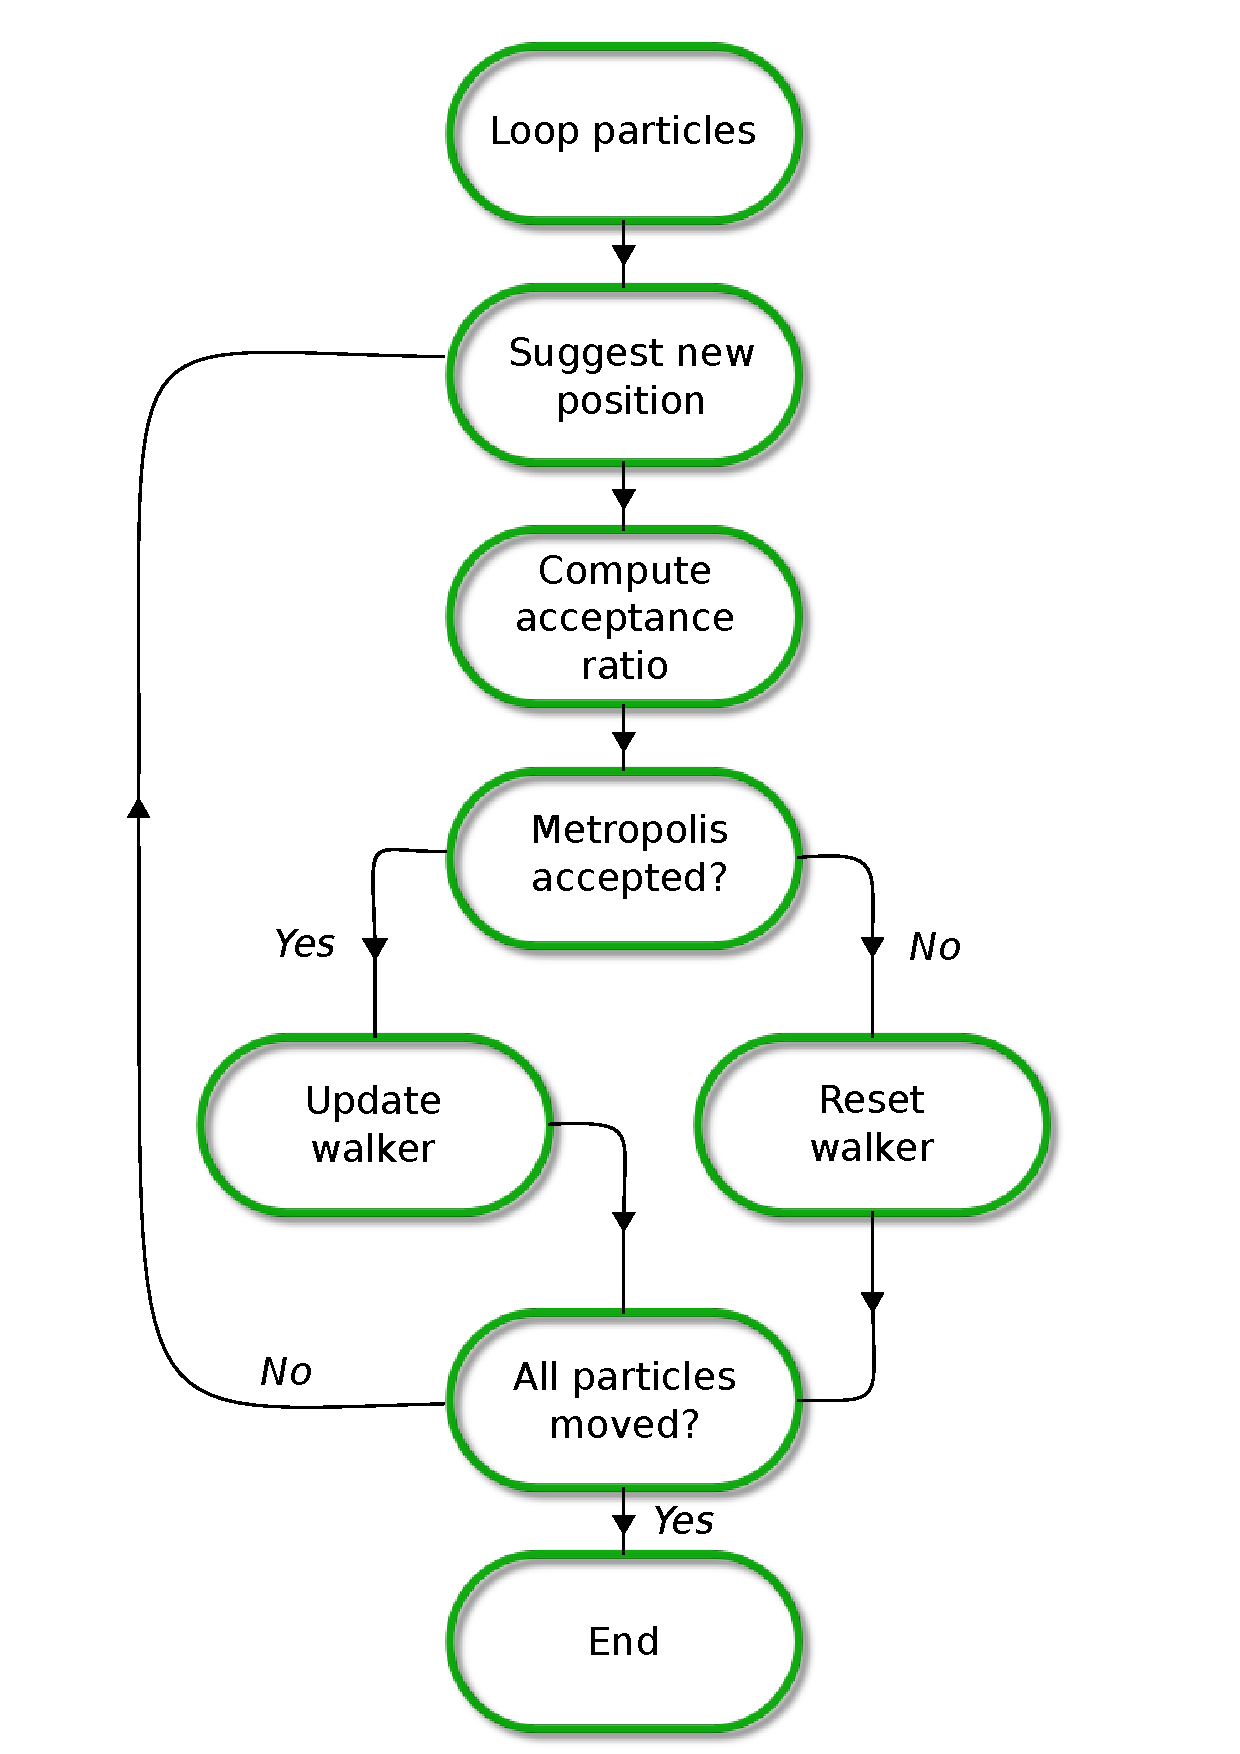
\includegraphics[scale=0.65]{../Graphics/DiffusionUML.pdf}
  \caption{Flow chart for iterating a walker through a single time step, i.e. simulation the application of the Green's function from Eq.~(\ref{eq:GDiff}) using the Metropolis algorithm. New positions are suggested according to the chosen diffusion model.}
 \end{center}
\end{figure}
\clearpage




\section{The Process of Branching}
\label{sec:branching}

The process of branching of Quantum Monte-Carlo is simulated by the creation or destruction of walkers with probability equal to that of the Green's function in Eq.~(\ref{eq:GB}) \cite{abInitioMC}. The explicit shapes in case of isotropic diffusion (ISO) and Anisotropic (FP) is

\begin{eqnarray}
 G_B^\mathrm{ISO}(i\,\rightarrow j) &=& e^{-\left(\frac{1}{2}\left[V(x_i) + V(x_j)\right] - E_T\right)\delta\tau} \\
 G_B^\mathrm{FP}(i\,\rightarrow j) &=& e^{-\left(\frac{1}{2}\left[E_L(x_i) + E_L(x_j)\right] - E_T\right)\delta\tau},
\end{eqnarray}

where $E_L(x_i)$ is the energy evaluated in configuration $x_i$ (see Section \ref{sec:calcExpVals} for details). 

As for all Green's functions, $G_B(i\,\rightarrow\,j) = 1$ implies no change. If the value is less than one, we have ``deaths'', i.e. the walker is removed from the ensemble. ``Births'' occur when the Green's function is greater than one; the walker is replicated.

The practical implementation becomes simply creating $\left[\mathrm{floor}(G_B) - 1\right]$ replicas of the current walker, with $\left[G_B - \mathrm{floor}(G_B)\right]$ probability of adding one extra on top (I skip the transition indices for now). As an example, a Green's function of $G_B=3.3$ will have guaranteed three replicas, however, there is a $3.3-3 = 0.3$ chance that one additional replica is made. The efficient comparison to do is to define 

\begin{equation}
\label{eq:gbMean}
 \overline{G}_B = \mathrm{floor}\left(G_B + a\right),
\end{equation}

where $a$ is a uniformly distributed number on $[0,1)$. The chance that $\overline{G}_B = G_B + 1$ is then equal to $\left[G_B - \mathrm{floor}(G_B)\right]$ as required. The three different scenarios which arise is

\begin{itemize}
 \item $\overline{G}_B = 1$ : No branching, proceed main loop.
 \item $\overline{G}_B = 0$ : The current walker is to be removed from the current ensemble.
 \item $\overline{G}_B > 1$ : Make $\overline{G}_B - 1$ replicas of the current walker.
\end{itemize}

This process is demonstrated in Fig. \ref{fig:branching}.

There are some programming challenges due to the fact that the number of walkers is not conserved, such as cleaning up dead walkers and stabilizing the population across different nodes. For details regarding this, see the actual code reference at ref. \cite{libBorealisCode}.

\begin{figure}
\label{fig:branching}
 \begin{center}
  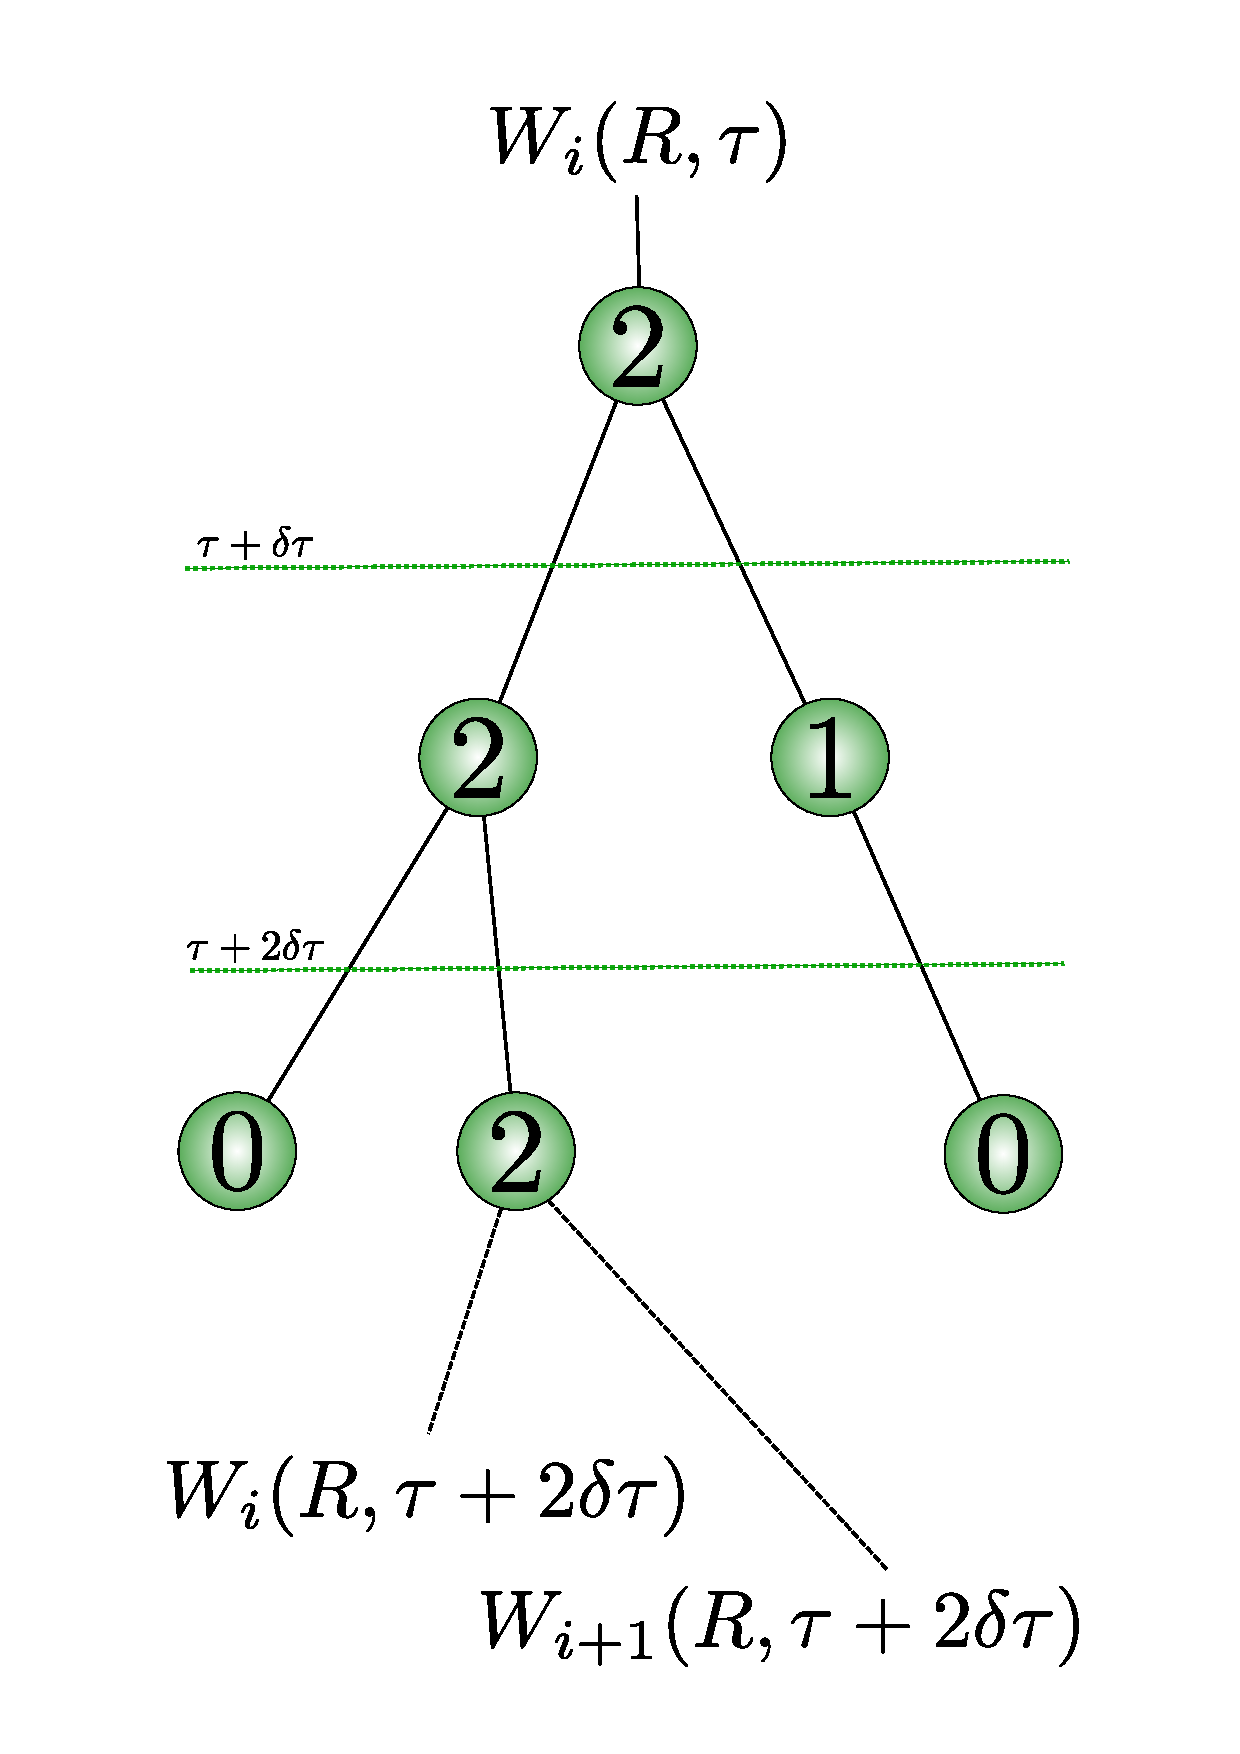
\includegraphics[scale=0.5]{../Graphics/branching.pdf}
  \caption{Branching illustrated. The initial walker $W_i(R, \tau)$ is branched according to the rules of Section \ref{sec:branching}. The numerical value inside the nodes represents $\overline{G}_B$ from Eq.~(\ref{eq:gbMean}). Each horizontal dashed line represent a diffusion step, i.e. a transition in time. Two lines exiting the same node represent identical walkers. After moving through the diffusion process, not two walkers should ever be equal (given that not all of the steps was rejected).}
 \end{center}
\end{figure}
\clearpage

\section{The Trial Wave Function}
\label{sec:trialWF}

Recall Eq.~(\ref{eq:schrodGeneralSolution})-(\ref{eq:schrodGeneralSolution2}). The initial condition, $\Phi(\vec r, t=0)$,
is in Quantum Monte-Carlo referred to as the trial wave function. Mathematically, we may choose any normalizable wave function, whose overlap with the exact ground state wave function, $\Psi_0(x)$, is non-zero. If the overlap is zero, that is, $C_0=0$ in Eq.~(\ref{eq:schrodGeneralSolution2}), the entire diffusion formalism breaks down, and no final state of convergence can be reached. On the other hand, the opposite scenario implies the opposite behavior; the closer $C_0$ is to unity, the more rapidly $\Psi_0(x)$ will become the dominant contribution to our distribution. 

Before getting into specifics, a few notes on many-body theory is needed. From this point on, all particles are assumed to be identical. For more information regarding basic Quantum Mechanics, I suggest reading ref. \cite{griffiths}. For mathematically rigid derivations of concepts, see ref. \cite{Sakurai:94}. More details regarding many-body theory can be found in ref. \cite{Shavitt}. 

\subsection{Many-body Wave Functions}
\label{sec:manyBodyWFs}

Many-body theory arise from the fact that we have \textit{many-body interactions}, e.g. the Coulomb interaction between two particles. If this was not the case, i.e. for non-interacting particles, the full system would decouple into $N$ single particle systems.

Finding the ground state is not surprisingly equivalent to solving the time-independent Schrödinger Equation

\begin{equation}
 \OP{H}\Psi_0(x) = E_0\Psi_0(x),
 \end{equation}
 
where $x \equiv \{x_1, x_2, ..., x_N\}$. Exact solutions to realistic many-body systems rarely exist, however, like in Section \ref{sec:statingDiff}, expanding the solution in a known basis is always legal, which reduces the problem into that of a \textit{coefficient hunt} 

\begin{equation}
\label{eq:manyBodyExp}
 \Psi_0(x) = \sum_{k=0}^\infty C_k'\Phi_k(x).
\end{equation}

Different many-body methods, e.g. \textit{Hartree Fock}\footnote{Hartree-Fock is roughly a basis change from the non-interacting case into a basis which is orthogonal to one-particle excitations. The exact ground state wave function should be orthogonal to all excited states, so it's a fair approximation depending on the dominance of one-particle excitations in the given system.} and genetic algorithms, give rise to different ways of hunting down these coefficients, however, certain concepts are necessarily common, for instance truncating the basis at some level, $K$:

\begin{equation}
\label{eq:manyBodyExpTrunc}
 \Psi_0(x) = \sum_{k=0}^K \tilde{C}_k'\Phi_k(x).
\end{equation}

The many-body basis elements $\Phi_k(x)$ are constructed using $N$ elements from a basis of single particle wave functions (or \textit{orbitals} for short), $\phi_n(x_i)$, combined in different ways. The process of calculating basis elements often boils down to a combinatoric exercise involving combinations of orbitals.

Imagine electrons surrounding a nucleus, i.e an atom; a single electron occupying state $n$ at a position $x_i$ is then described by the orbital $\phi_n(x_i)$. Each unique\footnote{Two wave functions are considered equal if they differ by nothing but a phase factor.} configuration of electrons will give rise to one unique $\Phi_k(x)$. In other words, the complete basis of $\Phi_k(x)$ is described by the collection of all possible excited states. $\Phi_0(x)$ is the ground state of the atom, $\Phi_1(x)$ has one electron exited to a higher shell, $\Phi_2(x)$ has another, and so on. See Fig.~\ref{fig:AtomicOrbitals} for a demonstration of this.

\begin{figure}
\label{fig:AtomicOrbitals}
 \begin{center}
  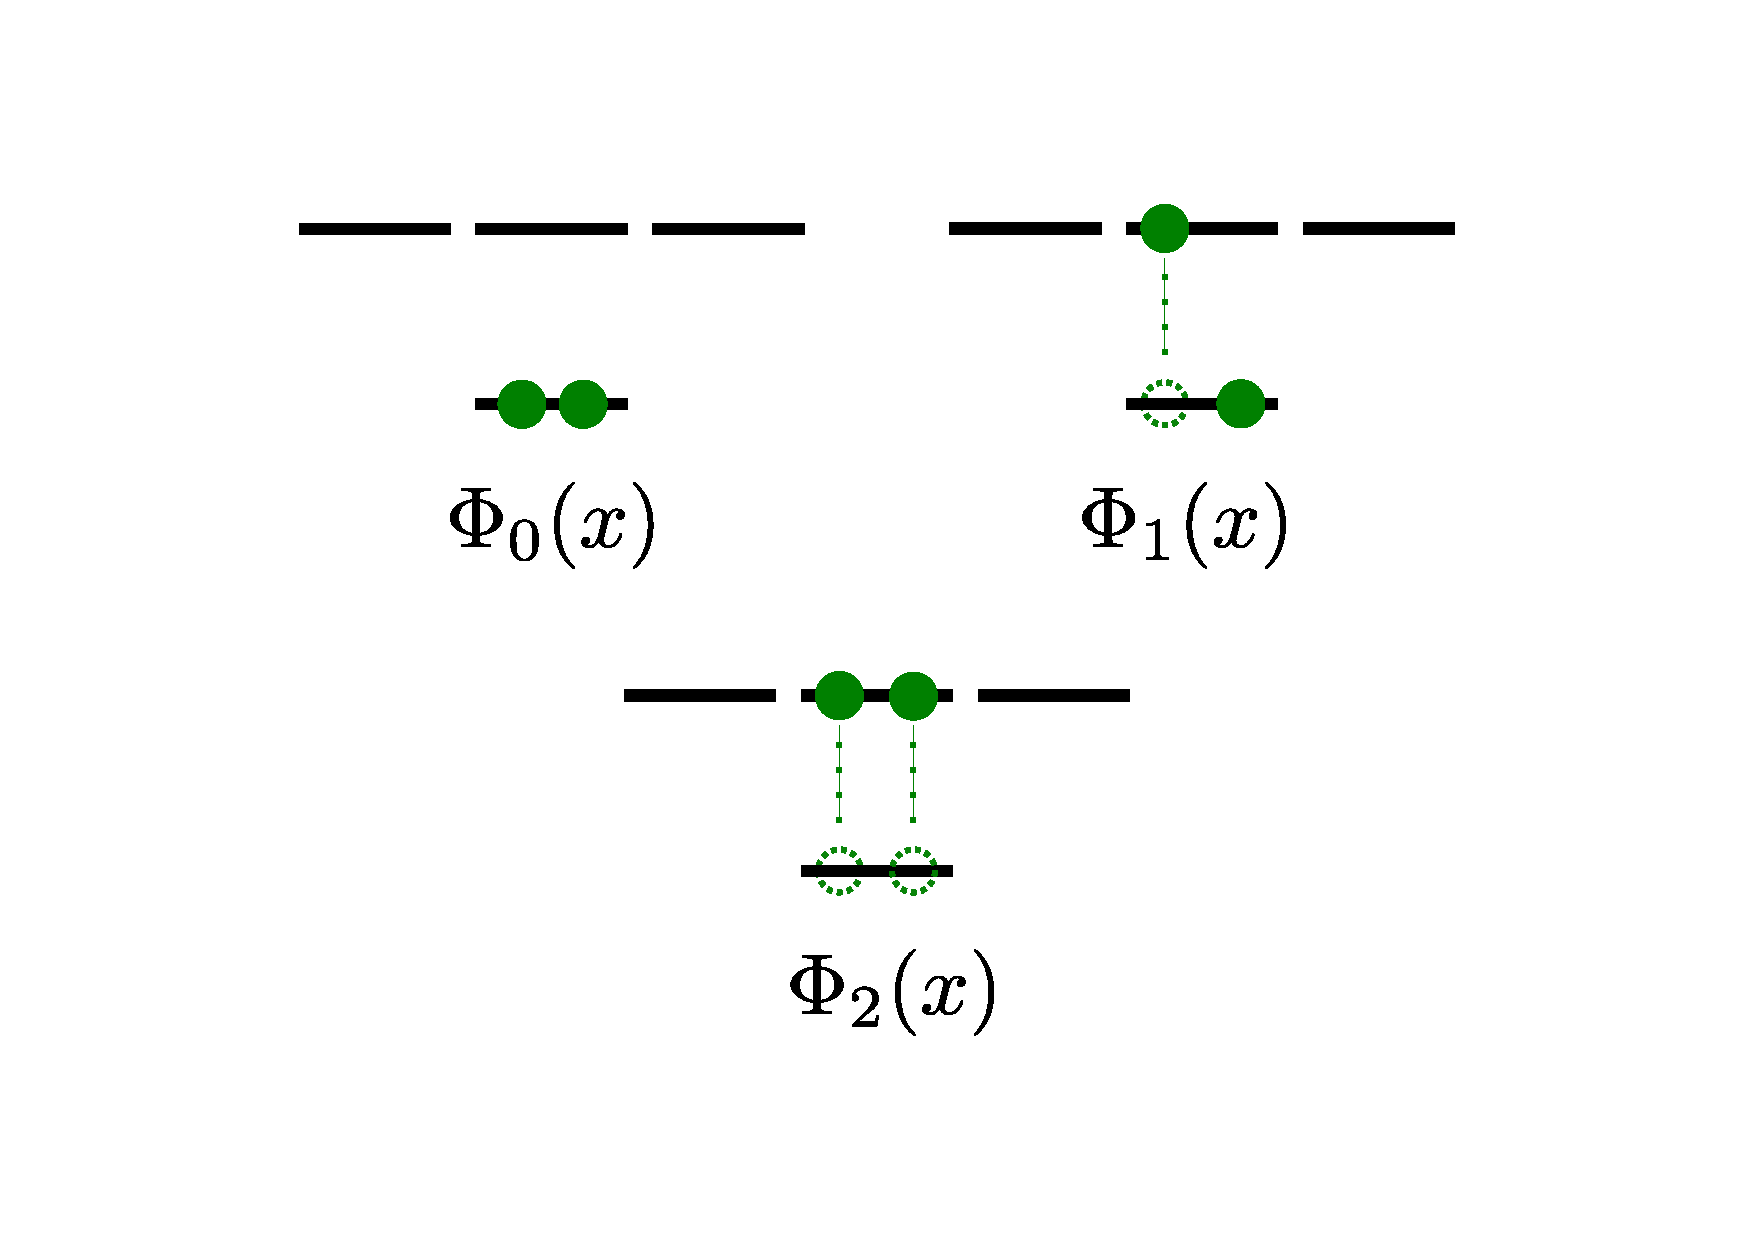
\includegraphics[scale=0.5]{../Graphics/shellStructure.pdf}
  \caption{Three different electron configurations in an shell structure making up three different $\Phi_k(x)$, i.e. constituents of the many-body basis described in Eq.~(\ref{eq:manyBodyExpTrunc}). An electron (solid dot) is represented by e.g. the orbital $\phi_{1s}(x_1)$.}
 \end{center}
\end{figure}

In other words, constructing a single solution of a many-body problem involves three steps:

\begin{center}
\begin{tabular}{l|l}
 Step one   &  Choose a set of orbitals $\phi_n(x_i)$. \\
 Step two   &  Construct $\Phi_k(x)$ from $N\times$ $\phi_n(x_i)$.   \\
 Step three &  Construct $\Psi_k(x)$ from $K\times$ $\phi_k(x)$.     \\
\end{tabular}
\end{center}

The last step is well described by Eq.~(\ref{eq:manyBodyExpTrunc}), but is seldom necessary to perform explicitly; expressions based on the calculated wave functions is given in terms of the constituents and their weights.

\subsubsection{Step one in detail}

The Hamiltonian for a $N$-particle system is 

\begin{equation}
 \OP{H} = \OP{H}_0 + \OP{H}_\mathrm{I},
\end{equation}

where $\OP{H}_0$ and $\OP{H}_\mathrm{I}$ are respectively the one-body and the many-body term. As an approximation, we truncate the many-body interactions at the Coulomb level. The one-body term consist of the external potential and the kinetic terms for all particles.

\begin{eqnarray}
 \OP{H}_0 &=& \sum_{i=1}^N \OP{h}_0(x_i) \\
          &=& \sum_{i=1}^N \OP{t}(x_i) + \OP{u}_\mathrm{ext}(x_i) \nonumber\\
 \OP{H}_\mathrm{I} &\simeq& \sum_{i<j=1}^N \OP{v}(r_{ij}) \\
          &=& \sum_{i<j=1}^N \frac{1}{r_{ij}}  \nonumber
\end{eqnarray}

The single particle orbitals are chosen to be the solutions of the non-interacting case (given that they exist)

\begin{equation}
\label{eq:orbitalEigenEq}
 \OP{h}_0(x_i)\phi_n(x_i) = \epsilon_n\phi_n(x_i).
\end{equation}

If no such choice can be made, choosing an generally suited basis, e.g. free-particle solutions, is the general strategy. 


\subsubsection{Step two in detail}

In the case of \textit{Fermions}, i.e. half-integer spin particles like electrons, protons, etc., $\Phi_k(x)$ is an anti-symmetric function\footnote{Interchanging two particles in an anti-symmetric wave function will reproduce the state changing only the sign.} on the form of a determinant: The \textit{Slater determinant}. The shape of the determinant is given in Eq.~(\ref{eq:SlaterDeterminantExplicit}). The anti-symmetry is a direct consequence of the \textit{Pauli Exclusion Principle}: At any given time, two fermions cannot occupy the same state. 

Bosons on the other hand, have symmetric wave functions (see Eq.~(\ref{eq:BosonicWFExplicit})), which in many ways are easier to deal with because of the lack of an exclusion principle. In order to keep the terminology less abstract and confusing, from here on, the focus will be on systems of fermions.

\begin{eqnarray}
\label{eq:SlaterDeterminantExplicit}
\Phi_0^\mathrm{AS}(x_1, x_2, ..., x_N) &\propto& \sum_\mathrm{P} (-)^\mathrm{P} \OP{P}\phi_1(x_1)\phi_2(x_2)\,...\,\phi_N(x_N) \nonumber\\
\nonumber\\
&=&\left| \begin{array}{cccc}
\phi_1(x_1) & \phi_2(x_1)& \cdots & \phi_N(x_1) \\
\phi_1(x_2) & \phi_2(x_2)& \cdots & \phi_N(x_2) \\
\vdots & \vdots& \ddots & \vdots \\
\phi_1(x_N) & \phi_2(x_N)& \cdots & \phi_N(x_N) \\
 \end{array} \right| \\
\nonumber\\
\nonumber\\
 \label{eq:BosonicWFExplicit}
 \Phi_0^\mathrm{S}(x_1, x_2, ..., x_N) &\propto& \sum_\mathrm{P} \OP{P}\phi_1(x_1)\phi_2(x_2)\,...\,\phi_N(x_N)
\end{eqnarray}

Comment to Eq.~(\ref{eq:SlaterDeterminantExplicit}) and Eq.~(\ref{eq:BosonicWFExplicit}): The permutation operator $\OP{P}$ is simply a way of writing \textit{in any combination of particles and states}, hence the combinatoric exercise mentioned previously.

\subsubsection{Dealing with correlations}

The contributions to the sum on the right-hand side in Eq.~(\ref{eq:manyBodyExp}) for $k>0$ are often referred to as \textit{correlation} terms. Given that the orbital wave functions are chosen by Eq.~(\ref{eq:orbitalEigenEq}), the existence of the correlation terms, i.e. $C_k' \ne 0$ for $k>0$, follows as a direct consequence of the many-body interaction, $H_\mathrm{I}$.

As an example, imagine performing an energy calculation with two particles being infinitely close; the Coulomb singularity will cause the energy to blow up. However, if we perform the calculation using the exact wave function, the diverging terms will cancel out; the energy is position independent. 

In other words, incorporating the correct correlated wave function will result in a cancellation in the diverging term as we approach singularities, a property which brings us closer to the exact wave function. 

These criteria are called \textit{Cusp Conditions}, and serve as a powerful guide when it comes to selecting a trial wave function. 

\subsection{Choice of Trial Wave function}

Choosing the trial wave function boils down to optimizing the overlap described in the introduction using a priori knowledge about the system at hand. As discussed previously, the optimal choice of single particle basis is eigenfunctions of the non-interacting case (given that they exist). Starting from Eq.~(\ref{eq:manyBodyExpTrunc}), the \textit{spatial wave function},the first step is to make sure the cusp conditions are obeyed.

Introducing the correlation functions $f(r_{ij})$, where $r_{ij}$ is the relative distance between particle $i$ and $j$, the general \textit{anzats} for the trial wave function becomes

\begin{equation}
\label{eq:firstAnzatsTWF}
 \Psi_T(x_1, ..., x_N) = \Big[\sum_{k=0}^K C_k\Phi_k(x_1, ..., x_N)\Big]\prod_{i<j}^Nf(r_{ij})
\end{equation}

\subsubsection{Explicit shapes}

Several models for the correlation function exist, however, some are less practical than others. An example given in ref. \cite{abInitioMC} demonstrates this nicely: Hylleraas presented the following correlation function 

\begin{equation}
 f(r_{ij})_\mathrm{Hylleraas} = e^{-\frac{1}{2} (r_i + r_j)}\sum_k d_k(r_{ij})^{a_k} (r_i + r_j)^{b_k}(r_i - r_j)^{e_k},
\end{equation}

where all $k$-subscripted parameters are free. Calculating the helium ground state energy using this correlation function with nine terms yields a four decimal precision. Eight digit precision is achieved by including almost 1078 terms. For the purpose of Quantum Monte-Carlo this is beyond overkill. 

A more well suited correlation function is the \textit{Padé Jastrow} function (skipping some redundant indices) 

\begin{eqnarray*}
 \prod_{i<j}^Nf(r_{ij}) &=& \exp(U) \\
         U &=&  \sum_{i<j}^N\left(\frac{\sum_k a_kr_{ij}^k}{1 + \sum_k \beta_kr_{ij}^k}\right) + \sum_i^N\left(\frac{\sum_k a'_kr_i^k}{1 + \sum_k \alpha_kr_i^k}\right).
\end{eqnarray*}

For systems where the correlations are well behaving, it is custom to drop the second term, and keep only the $k=1$ term, i.e.

\begin{equation}
 \label{eq:jastrow}
 f(r_{ij}; \beta) = \exp\left(\frac{a_{ij} r_{ij}}{1 + \beta r_{ij}}\right),
\end{equation}

where $\beta$ is a variational parameter, and $a_{ij}$ is a spin-dependent constant tuned to obey the cusp condition.

Shifting the focus back to the spatial wave function, in the case of a fermionic system, the evaluation of a $N\times N$ Slater determinant is holding back the effectiveness of many-particle simulations. However, assuming we have a spin-independent Hamiltonian, we can split the spatial wave function is two; one part for each spin eigenvalue. A detailed derivation of this is given in the appendix of ref. \cite{QMCPHD2008}. Assuming spin-half particles we get

\begin{equation}
 \Psi_T(x_1, ..., x_N; \beta) = \Big[\sum_{k=0}^K C_k\tilde\Phi_k(x_1, ..., x_{\frac{N}{2}})\tilde\Phi_k(x_{\frac{N}{2}-1}, ..., x_{N})\Big]\prod_{i<j}^Nf(r_{ij}; \beta).
\end{equation}

Since the particles are identical, we are free to say that the first half are spin up, and the second spin down, hence the splitting as above. For simplicity, the spin up determinant will from here on be labeled $D^\uparrow$, and the spin down one $D^\downarrow$. Stitching everything together yields the following explicit shape for a spin-independent Hamiltonian using a one-parameter Padé Jastrow function

\begin{equation}
\label{eq:MultiDeterminantTWF}
 \Psi_T(x_1, ..., x_N; \beta) = \sum_{k=0}^K C_kD^\uparrow_kD^\downarrow_k\prod_{i<j}^Nf(r_{ij}; \beta).
\end{equation}

This shape is referred to as a \textit{Multi-determinant} trial wave function. 

\subsubsection{Limitations}

Depending on the complexity of the system at hand, we need more complicated trial wave functions. However, it is important to distinguish between simply integrating a trial wave function, and performing the full diffusion calculation. As a reminder: Simple integration will not be able to tweak the distribution; what you have is what you get. Solving the diffusion problem, on the other hand, will alter the distribution from that of the trial wave function ($t = 0$) into a distribution closer to the exact wave function by Eq.~(\ref{eq:schrodGeneralSolution2}). 

Because of this fact, our limitations due to the trial wave function is far less than what is the case of standard Monte-Carlo integration. A heavier trial wave function might convergence faster, but at the expense of being more CPU-intensive. This means that we are in a position to trade CPU-time per walker for convergence time. For systems of many particles, CPU-time per walker needs to be as low as possible in order to get the computation done in a reasonable amount of time, i.e., the choice of trial wave function needs to be done in light of the system at hand, and the specific aim of the computation. 

In the case of well-behaving systems, a single determinant converges rapidly enough. This simplicity opens up the possibility of simulating large systems efficiently. This will be referred to as a \textit{single determinant} trial wave function, and serve as a  very simple approximation. In order to optimize the overlap with the exact wave function, a variational parameter $\alpha$ is introduced in the spatial part (from  Eq.~(\ref{eq:jastrow}), we already have $\beta$)

\begin{equation}
\label{eq:singleDeterminantTWF}
 \Psi_T(x_1, ..., x_N; \alpha, \beta) = D^\uparrow(\alpha)D^\downarrow(\alpha)\prod_{i<j}^Nf(r_{ij}; \beta).
\end{equation}

Determining optimal values for the variational parameters will be discussed in Section \ref{sec:selectingOptVarPar}.

\subsection{Calculating Expectation Values}
\label{sec:calcExpVals}

The expectation value of an operator $\OP{O}$ is sampled through \textit{local} values, $O_L(x)$

\begin{eqnarray}
 \bra{\Psi_T}\OP{O}\ket{\Psi_T} &=& \int \Psi_T(x)^\ast \OP{O} \Psi_T(x)\mathrm{d}x \nonumber\\
                                &=& \int |\Psi_T|^2\left(\frac{1}{\Psi_T(x)}\OP{O}\Psi_T(x)\right)\mathrm{d}x \nonumber\\
                                &=& \int |\Psi_T|^2 O_L(x)\mathrm{d}x \\
                         O_L(x) &=& \frac{1}{\Psi_T(x)}\OP{O}\Psi_T(x)           
\end{eqnarray}

Discretizing the integral (and thus introducing an error) yields 

\begin{equation}
 \bra{\Psi_T}\OP{O}\ket{\Psi_T} \equiv \Exp{O} \simeq \frac{1}{n}\sum_{i=1}^n O_L(x_i) \equiv \overline{O},
\end{equation}

where $x_i$ is a random variable following the distribution of the trial wave function. The \textit{ensemble average},  $\Exp{O}$ will, given ergodicity, equal the estimated average $\overline{O}$ in the limit $n\rightarrow\infty$, i.e.

\begin{equation}
 \label{eq:MeanVStrueExp}
 \Exp{O} = \lim_{n\to\infty} \overline{O} = \lim_{n\to\infty}\frac{1}{n}\sum_{i=1}^n O_L(x_i)
\end{equation}


In the case of the energy estimation, this means that once our walkers hit equilibrium, we can start sampling local values based on their configurations $x_i$. In the case of energies, we get

\begin{equation}
 \langle E \rangle \simeq \frac{1}{n}\sum_{i=1}^n \left(\frac{1}{\Psi_T(x_i)}\left(-\frac{1}{2}\nabla^2\right)\Psi_T(x_i) + V(x_i)\right)
\end{equation}

\subsection{Normalization}

Every explicit calculation using the trial wave function in Quantum Monte-Carlo involves taking ratios. Ratios implies cancellation of the normalization factors. Eq.~(\ref{eq:MetroGeneralGreen}) from the Metropolis section, the Quantum Force in the Fokker-Planck equation, and the sampling of local values describes in the previous section demonstrates exactly this; everything involves ratios.

Not having to normalize our wave functions saves us a lot of CPU-time, but it also relieves us of complicated normalization factors in our single particle basis expressions; any constants multiplying $\phi_n(x_i)$ in Eq.~(\ref{eq:SlaterDeterminantExplicit}) and Eq.~(\ref{eq:BosonicWFExplicit}), can be taken outside the sum over permutations, and will hence cancel when the ratio between two wave functions constituting of the same single particle orbitals are computed (note: Single determinant only). 

In the case of multi-determinants trial wave functions, the normalization factors from the single particle basis elements  will be absorbed by the respective determinant's coefficient $C_k$, and is hence obsolete in this case as well.


\subsection{Selecting Optimal Variational Parameters}
\label{sec:selectingOptVarPar}

All practical ways of determining the optimal values of the variational parameters originate from the same powerful principle: \textit{The Variational Principle}. The easiest way of demonstrating the principle is to evaluate the expectation value of the energy, using an approach similar to what used in Eq.~(\ref{eq:schrodGeneralSolution2})

\begin{eqnarray*}
 E_0 &=& \bra{\Psi_0}\OP{H}\ket{\Psi_0}  \\
 E   &=& \bra{\Psi_T(\alpha, \beta)}\OP{H}\ket{\Psi_T(\alpha, \beta)}\\
     &=& \sum_{kl} C_k^\ast C_l \underbrace{\bra{\Psi_k}\OP{H}\ket{\Psi_l}}_{E_k\delta_{kl}} \\
     &=& \sum_k |C_k|^2E_k
\end{eqnarray*}

Using further that $E_0$ is the lowest energy eigenvalue, we can, just as done with the time propagator, introduce $E_k = E_0 + \delta E_k$ to simplify the arguments

\begin{eqnarray*}
 E   &=& \sum_k |C_k^2| (E_0 + \delta E_k) \\
     &=& E_0 \underbrace{\sum_k |C_k^2|}_{1} + \underbrace{\sum_k |C_k|^2\delta E_k}_{\ge 0} \\
     &\ge& E_0
\end{eqnarray*}

The conclusion is stunning: No matter how we choose our trial wave function, we will never undershoot the exact ground state energy. This basically means that the problem of choosing variational parameters boils down to a minimization problem in the parameters space (we assume no maximum exist for finite parameter values)

\begin{equation}
\label{eq:varMin}
\frac{\partial \langle E\rangle}{\partial \alpha_i} = \frac{\partial}{\partial \alpha_i}\bra{\Psi_T(\alpha_i)}\OP{H}\ket{\Psi_T(\alpha_i)} = 0
\end{equation}

In order to work with Eq.~(\ref{eq:varMin}) in practice, we need to rewrite it in terms of known values. Since our wave function is dependent on the variational parameter, we need to include the expression for the normalization factor before we can expand the expression

\newcommand{\Norm}{\braket{\Psi_T(\alpha_i)}{\Psi_T(\alpha_i)}}

\begin{eqnarray*}
 \frac{\partial \langle E\rangle}{\partial \alpha_i}  &=& \frac{\partial}{\partial \alpha_i} \frac{\bra{\Psi_T(\alpha_i)}\OP{H}\ket{\Psi_T(\alpha_i)}}{\Norm} \\
 &=& \frac{\left(\bra{\Psi_T(\alpha_i)}\frac{\partial}{\partial \alpha_i}\OP{H}\ket{\Psi_T(\alpha_i)} + \bra{\Psi_T(\alpha_i)}\OP{H}\frac{\partial}{\partial \alpha_i}\ket{\Psi_T(\alpha_i)}\right)}{\Norm^2}\Norm \\
 &-& \bra{\Psi_T(\alpha_i)}\OP{H}\ket{\Psi_T(\alpha_i)}\frac{\left(\bra{\Psi_T(\alpha_i)}\frac{\partial}{\partial \alpha_i}\right)\ket{\Psi_T(\alpha_i)} + \bra{\Psi_T(\alpha_i)}\left(\frac{\partial}{\partial \alpha_i}\ket{\Psi_T(\alpha_i)}\right)}{\Norm^2},\\
\end{eqnarray*}

where the product and division rules for derivatives have been applied. The Hamiltonian does not depend on the variational parameters, and hence both terms in the first expansion is equal. Cleaning up the expression yields

\begin{eqnarray}
 \frac{\partial \langle E\rangle}{\partial \alpha_i} &=& 2\left(\frac{\bra{\Psi_T(\alpha_i)}\OP{H}\frac{\partial}{\partial \alpha_i}\ket{\Psi_T(\alpha_i)}}{\Norm} - \langle E \rangle\frac{\bra{\Psi_T(\alpha_i)}\frac{\partial}{\partial \alpha_i}\ket{\Psi_T(\alpha_i)}}{\Norm} \right) \nonumber \\
  &=& 2\left(\left< E \frac{\partial \Psi_T}{\partial \alpha_i} \right> -\left< E\right>\left<\frac{\partial \Psi_T}{\partial \alpha_i} \right> \right) \label{eq:varParGrad}
\end{eqnarray}

Using this expression for the \textit{variational gradient} means we can calculate the derivatives exactly the same way we calculate the energy, and use these derivatives to move in the direction of the variational minimum in Eq.~(\ref{eq:varMin}). 

This strategy give rise to numerous ways of finding the optimal parameters, such as using the well known Newton's method, conjugate gradient methods \cite{golub1996matrix}, steepest descent (similar to Newton's method), and many more. 
The method implemented for this thesis is called \textit{Adaptive Stochastic Gradient Descent}, and is an efficient iterative algorithm for seeking the variational minimum. 

\section{Gradient Descent}

The direction of a gradient serves as a guide to extremal values. In the case of the Quantum Force, it leads the walker to regions of high probability, and in the case of \textit{Gradient Descent} methods, it reveals function minima. The Adaptive Stochastic Gradient Descent (ASGD) algorithm is best understood from it's basic predecessor

\subsection{General Gradient Descent}

Seeking maxima or minima is simply a question of whether the positive or negative direction of the gradient is followed.
Imagine a function, $f(x)$, with a minimum residing at $x=x_m$. The information at hand is then

\begin{eqnarray}
 \nabla f(x_m) &=& 0 \\
 \nabla f(x_m - \mathrm{d}x) &<& 0 \\
  \nabla f(x_m + \mathrm{d}x) &>& 0
\end{eqnarray}

where $\mathrm{d}x$ is a infinite decimal displacement. 

\begin{figure}
\label{fig:SGD}
 \begin{center}
  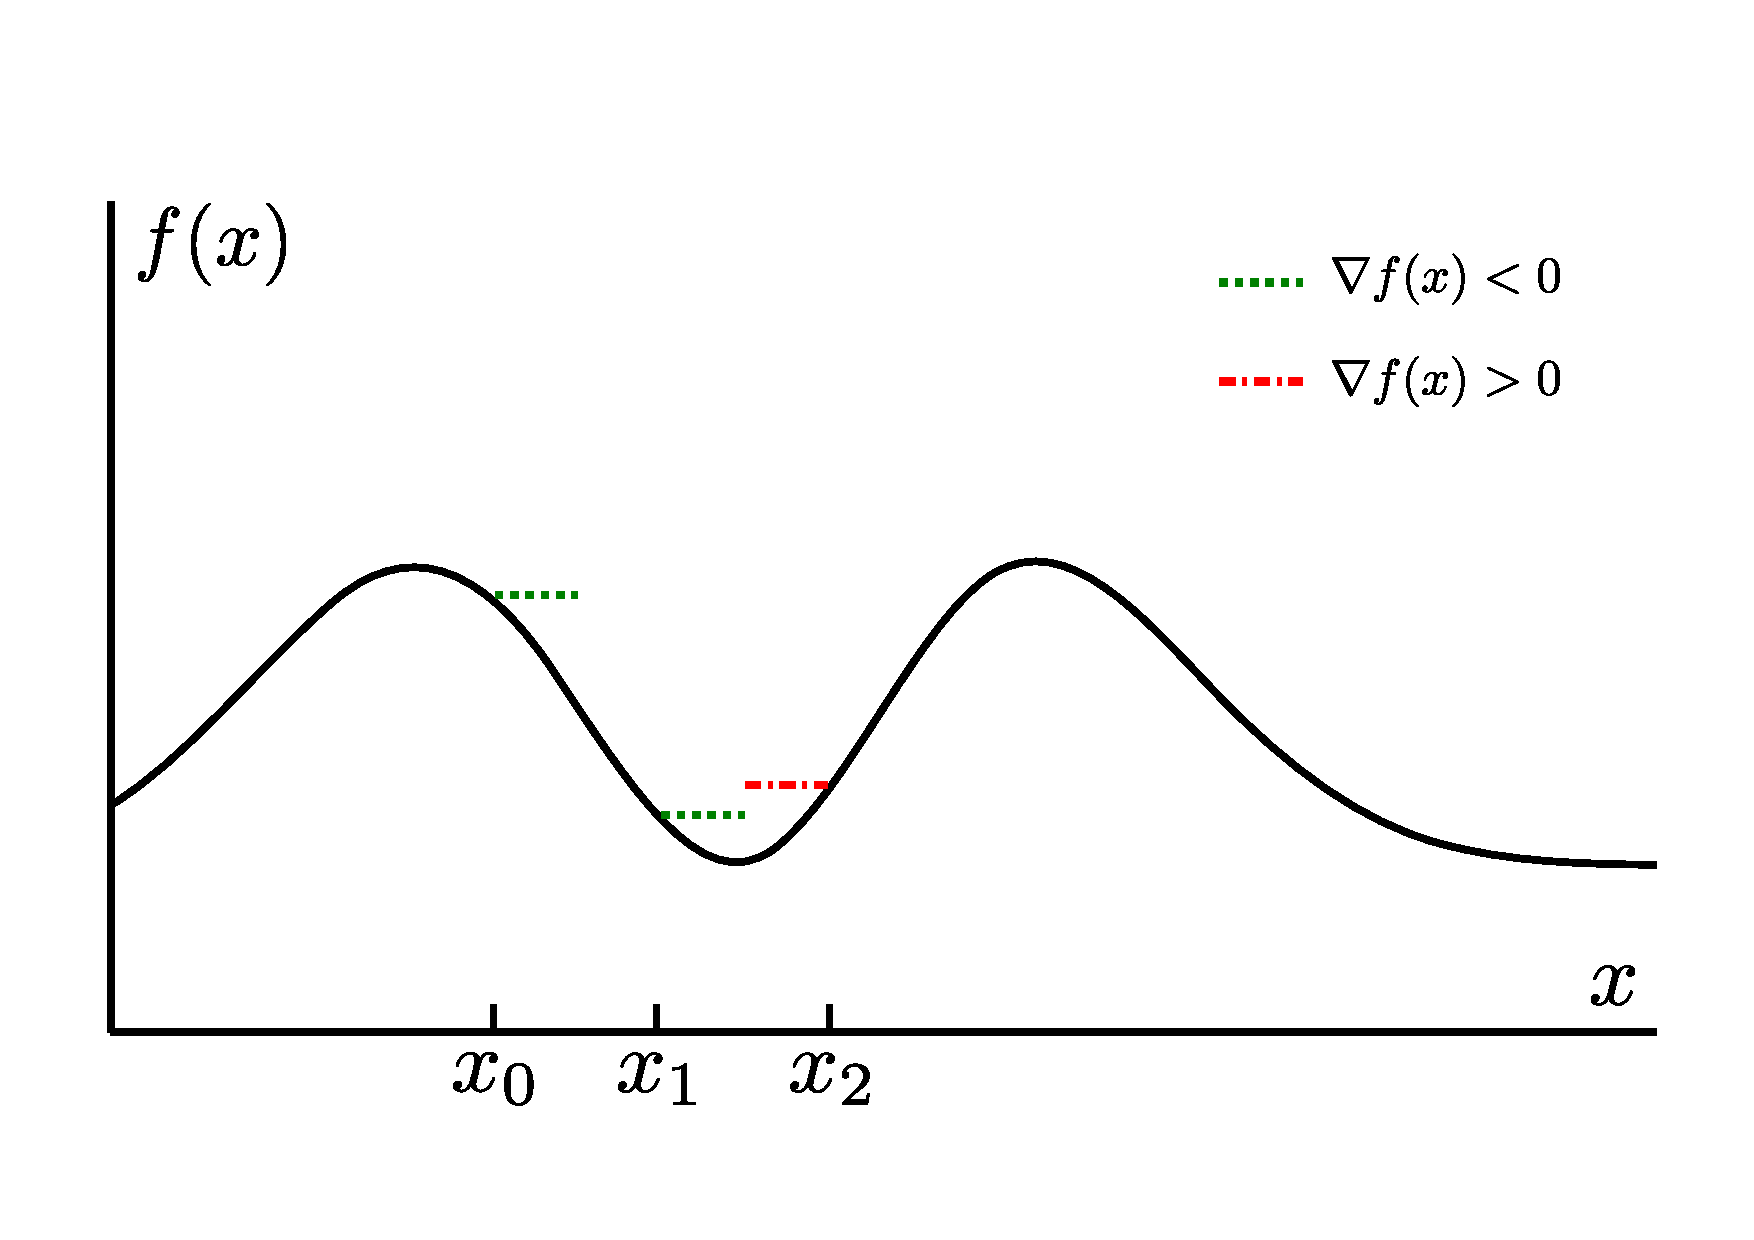
\includegraphics[scale=0.3]{../Graphics/SGD.pdf}
  \caption{Two steps of a one dimensional Gradient Descent process. Steps are taken in the direction of the negative gradient (indicated by dotted lines).}
 \end{center}
\end{figure}

Assume now that we start from an initial position $x_0$, and measure the direction of the gradient before we take a step in that direction. From Fig. \ref{fig:SGD} and the previous equations, we see that once we cross the minimum, the gradient changes sign. The brute force way of minimizing is to stop once the gradient changes sign, however, this would require extremely many extremely small steps in order to achieve good precision. The difference equation for the brute force case would be

\begin{equation}
 x_{i+1} = x_i - \delta\frac{\nabla f(x_i)}{|\nabla f(x_i)|}
\end{equation}


A better algorithm is to continue iterating even though the minimum is crossed. The brute force scheme breaks down in this case, oscillating between two points, e.g. $x_1$ and $x_2$ in Fig. \ref{fig:SGD}, because of the constant step length $\delta$. To counter this, a changing step length $\delta_i$ is introduced

\begin{equation}
\label{eq:SGD}
  x_{i+1} = x_i - \delta_i\nabla f(x_i)
\end{equation}

All Gradient/Steepest Descent methods is in principle described by Eq.~(\ref{eq:SGD}). Some examples are

\begin{listliketab}
\storestyleof{itemize}
 \begin{tabular}{l l}
  \textbullet  \,Brute Force I   &  $\delta_i = \delta \frac{1}{|\nabla f(x_i)|}$ \\
  \textbullet  \,Brute Force II  &  $\delta_i = \delta $ \\
  \textbullet  \,Brute Force III &  $\delta_i = \delta / i^{2}$ \\
  \textbullet  \,Newton's Method &  $\delta_i = \frac{1}{\nabla^2 f(x_i)}$\\
 \end{tabular}
\end{listliketab}

Iterative gradient methods will only reveal one local extrema, depending on the choice of $x_0$ and $\delta$. In order to find several extrema, multiple unique processes can be run. Calculating the local gradient is simply a finite difference calculation (assuming the analytic expression is not known).

\subsection{Stochastic Gradient Descent}

Minimizing stochastic quantities, such as the variance or expectation values, adds another layer of complications on top of the methods described in the previous section. Assuming a closed form expression for the stochastic quantity is unobtainable, the gradient needs to be calculated by using e.g. Monte-Carlo sampling. Eq.~(\ref{eq:varParGrad}) is an example of such a process.

A full precise sampling of the stochastic quantities are expensive and unpractical. Stochastic Gradient methods use different techniques in order to make the sampling more effective, such as multiple walkers, thermalization, and more. Using a finite difference scheme with stochastic quantities are dangerous, as uncertainties in the values will cause the gradient to become unstable when the variations are low (close to the minimum). This is illustrated in Fig. \ref{fig:sSGD}.

\begin{figure}
\label{fig:sSGD}
 \begin{center}
  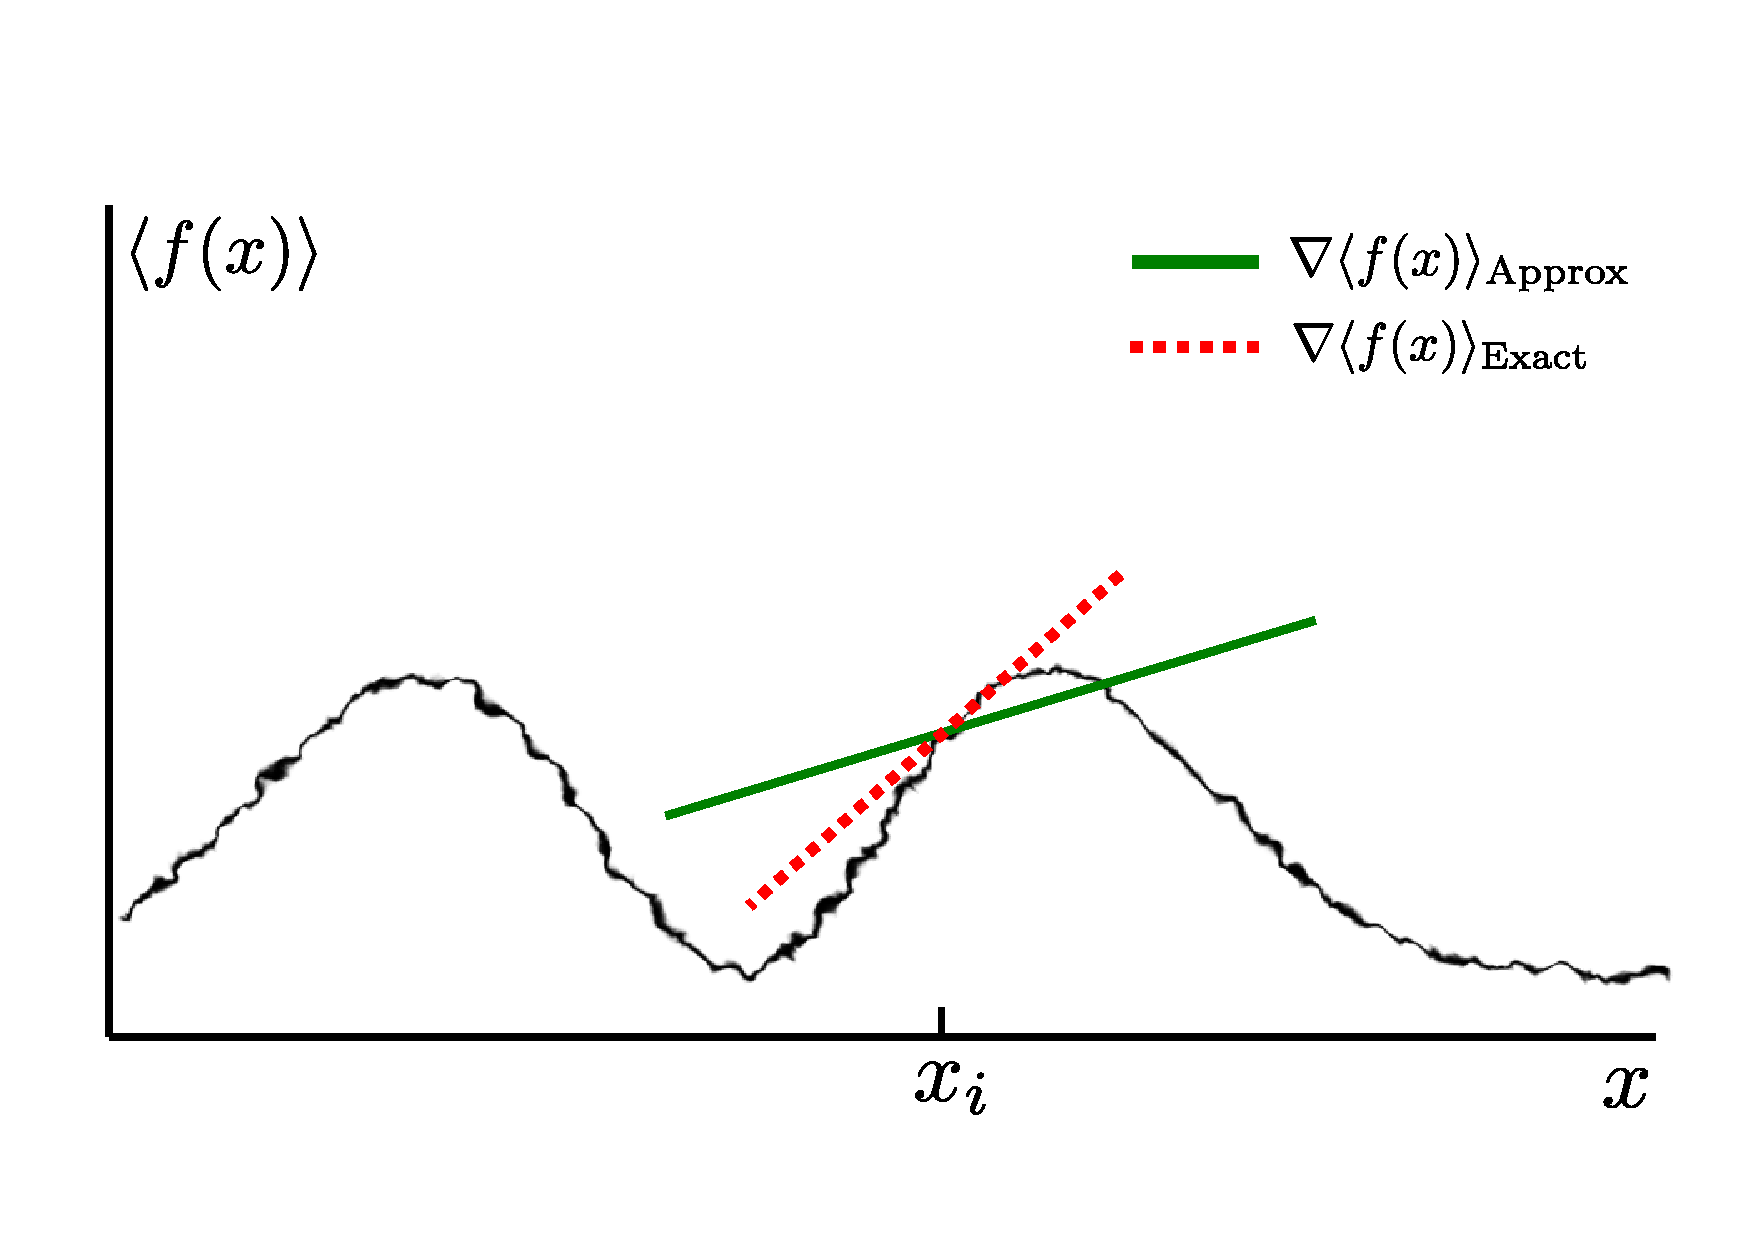
\includegraphics[scale=0.3]{../Graphics/SSGD.pdf}
  \caption{A one dimensional plot of an expectation valued function. Smeared lines are representing uncertainties due to rough sampling. The direction of the local gradient (solid green line) at a point $x_i$ is not necessarily a good estimate of the actual analytic gradient (dashed red line).}
 \end{center}
\end{figure}


\subsection{Adaptive Stochastic Gradient Descent}

Adaptive Stochastic Gradient Descent (ASGD) has it's roots in the mathematics of automated control theory \cite{ASGD_MB}. The automated process, is that of choosing an optimal step length $\delta_i$ for the current transition $x_{i}\to x_{i+1}$. This process is based on the inner product of the old and the new gradient though a variable 

\begin{equation}
\label{eq:ASGD_X_i}
 X_i \equiv -\nabla_i\cdot \nabla_{i-1}
\end{equation}

The step length from Eq.~(\ref{eq:SGD}) is in ASGD modeled in the following manner

\begin{eqnarray}
 \delta_i   &=& \gamma(t_i) \\
 \gamma(t)  &=& a/(t + A) \label{eq:ASGD_delta_i}\\
 t_{i+1}    &=& \max(t_i + f(X_i), 0) \label{eq:ASGD_t_i}\\
 f(x)       &=& f_\mathrm{min} + \frac{f_\mathrm{max} - f_\mathrm{min}}{1 - (f_\mathrm{max}/f_\mathrm{min})e^{-x/\omega}}\label{eq:ASGD_f_i}
\end{eqnarray}

with $f_\mathrm{max} > 0$, $f_\mathrm{min} < 0$, and $\omega > 0$. Free parameters are $a$, $A$, $t_0$, however, Ref. \cite{ASGD} suggests $A=20$ and $t_0=t_1=A$ for universal usage.

Notice that the step length increase if $t_i$ decrease and vice-versa. A smaller step length is sought for regions close to the minimum. The function of $f(x)$ is to alter the step length by changing the trend of $t$. If we are close to the minimum, a smaller step length is sought, and hence $t$ must increase. We know from previous discussion, that if the sign of the gradient change, we have crossed the minimum. Crossing the minimum with ASGD has the following consequence

\begin{itemize}
 \item Eq.~(\ref{eq:ASGD_X_i}): The value of $X_i$ will be positive.
 \item Eq.~(\ref{eq:ASGD_f_i}): $f(X_i)$ will return a value in $[0, f_\mathrm{max}]$ depending on the magnitude of $X_i$ .
 \item Eq.~(\ref{eq:ASGD_t_i}): The value of $t$ will increase, i.e. $t_{i+1} > t_i$ .
 \item Eq.~(\ref{eq:ASGD_delta_i}): The step length will decrease .
\end{itemize}

The second step regarding $f(X_i)$ can be visualized in Fig. \ref{fig:f_ASGD}.

\begin{figure}
\label{fig:f_ASGD}
 \begin{center}
  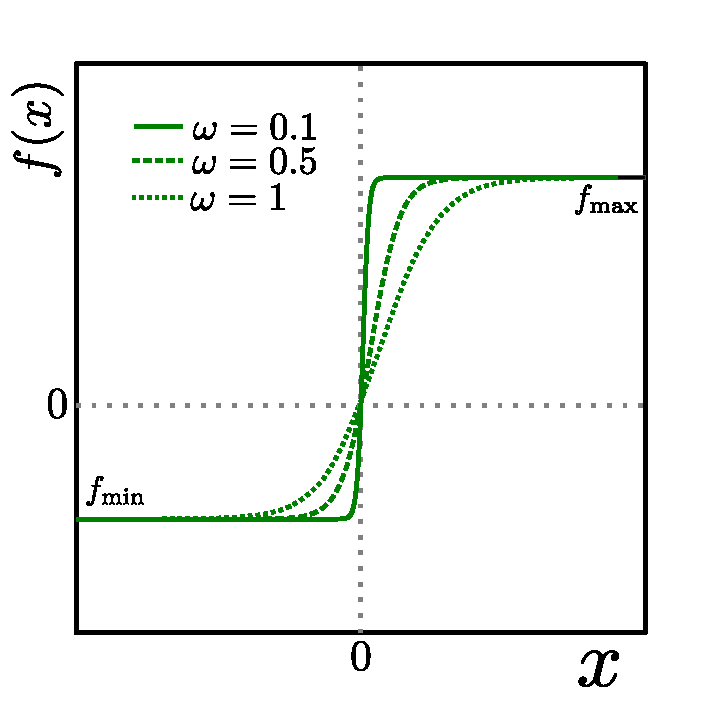
\includegraphics[scale=0.75]{../Graphics/ASGD_f.pdf}
  \caption{Examples of $f(X_i)$ as published in ref. \cite{ASGD}. As $\omega\to0$, $f(x)$ approaches a step function.}
 \end{center}
\end{figure}

\subsubsection{Assumptions}
\begin{itemize}
 \item The statistical error in the sampled gradients are distributed with zero mean.
\end{itemize}

This is shown in ref. \cite{ASGD} to be true; they are normally distributed. The implication is that upon combining gradient estimates for $N$ different processes, the accumulative error will tend to zero quickly.

\begin{itemize}
 \item The step length $\gamma(t)$ is a positive monotone decreasing function defined on $[0,\infty)$ with maximum at $t=0$.
\end{itemize}

With $\gamma(t)$ being as in Eq~(\ref{eq:ASGD_delta_i}), this is easily shown.

\begin{itemize}
 \item The function $f(x)$ is continuous and monotone increasing with $f_\mathrm{min} = \displaystyle\lim_{x\to\infty} f(x)$ and $f_\mathrm{max} =  \displaystyle\lim_{x\to-\infty} f(x)$.
\end{itemize}

This is exactly the behavior displayed in Fig. \ref{fig:f_ASGD}.


These assumptions and several more are described in more detail in ref. \cite{ASGD}. They underline that the shape and flow of the algorithm is in no way random; ASGD is optimizing minimization of stochastic quantities. 

\subsubsection{Implementation}

A flow chart of the implementation is given in Fig. \ref{fig:ASGD_flow}. For specific details regarding the implementation, i refer to the code \cite{libBorealisCode}. An example of minimization using ASGD is given in Fig. \ref{fig:ASGD_Ex}. 

\begin{figure}
\label{fig:ASGD_Ex}
 \begin{center}
  \subfigure{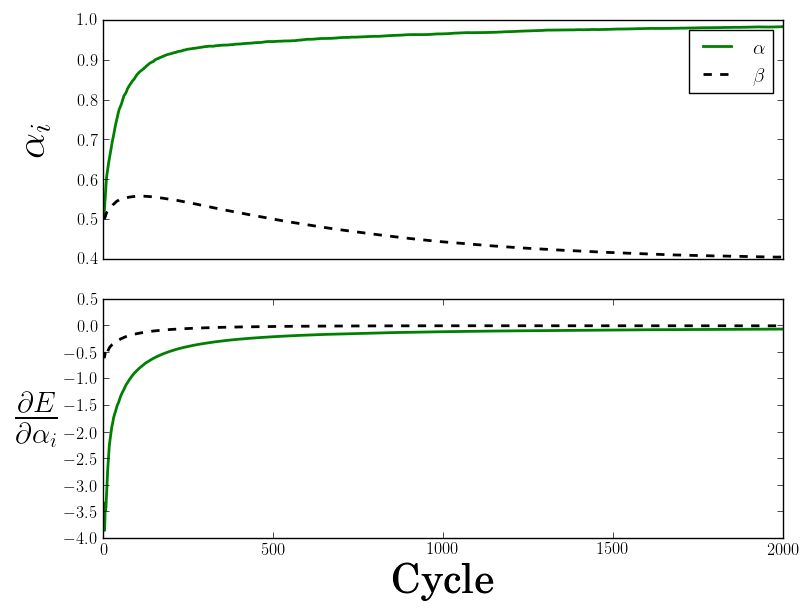
\includegraphics[scale=0.37]{../Graphics/ASGD_min_paramGrad_ex.png}}
  \subfigure{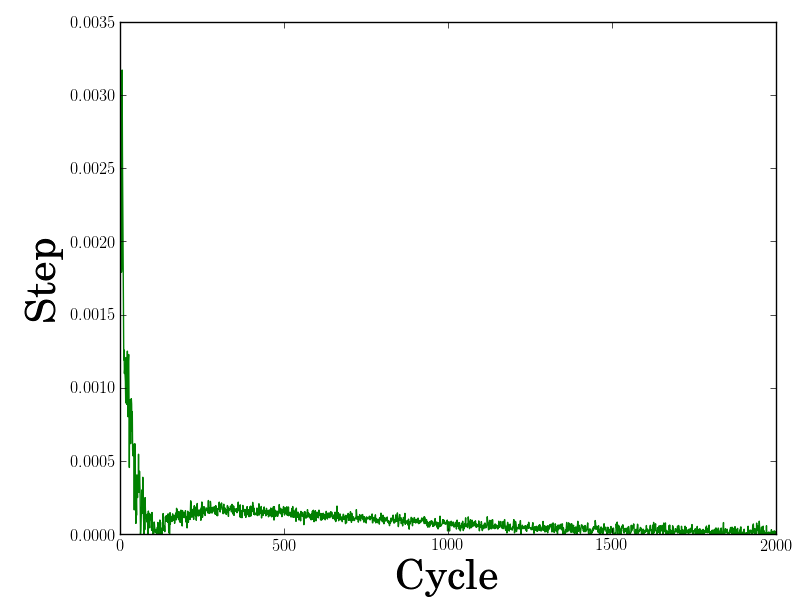
\includegraphics[scale=0.37]{../Graphics/ASGD_min_step_ex.png}} 
  \caption{Results of Adaptive Stochastic Gradient Descent used on a two-particle Quantum Dot with unit oscillator frequency using $400$ cycles pr. gradient sampling and $40$ independent walkers. The right figure shows the evolution of the time step. The left figure shows the evolution of the variational parameters $\alpha$ and $\beta$ introduced in Section \ref{sec:trialWF} on top, and the evolution of the gradients on the bottom. The gradients are cycle averaged to reveal the pattern underlying the noise. We clearly see that they tend to zero, $\beta$ somewhat before $\alpha$. The step rushes to zero; we get a small rebound in the step after forcing it zero as it attempts to cross to negative values.}
 \end{center}
\end{figure}


\begin{figure}
\label{fig:ASGD_flow}
 \begin{center}
  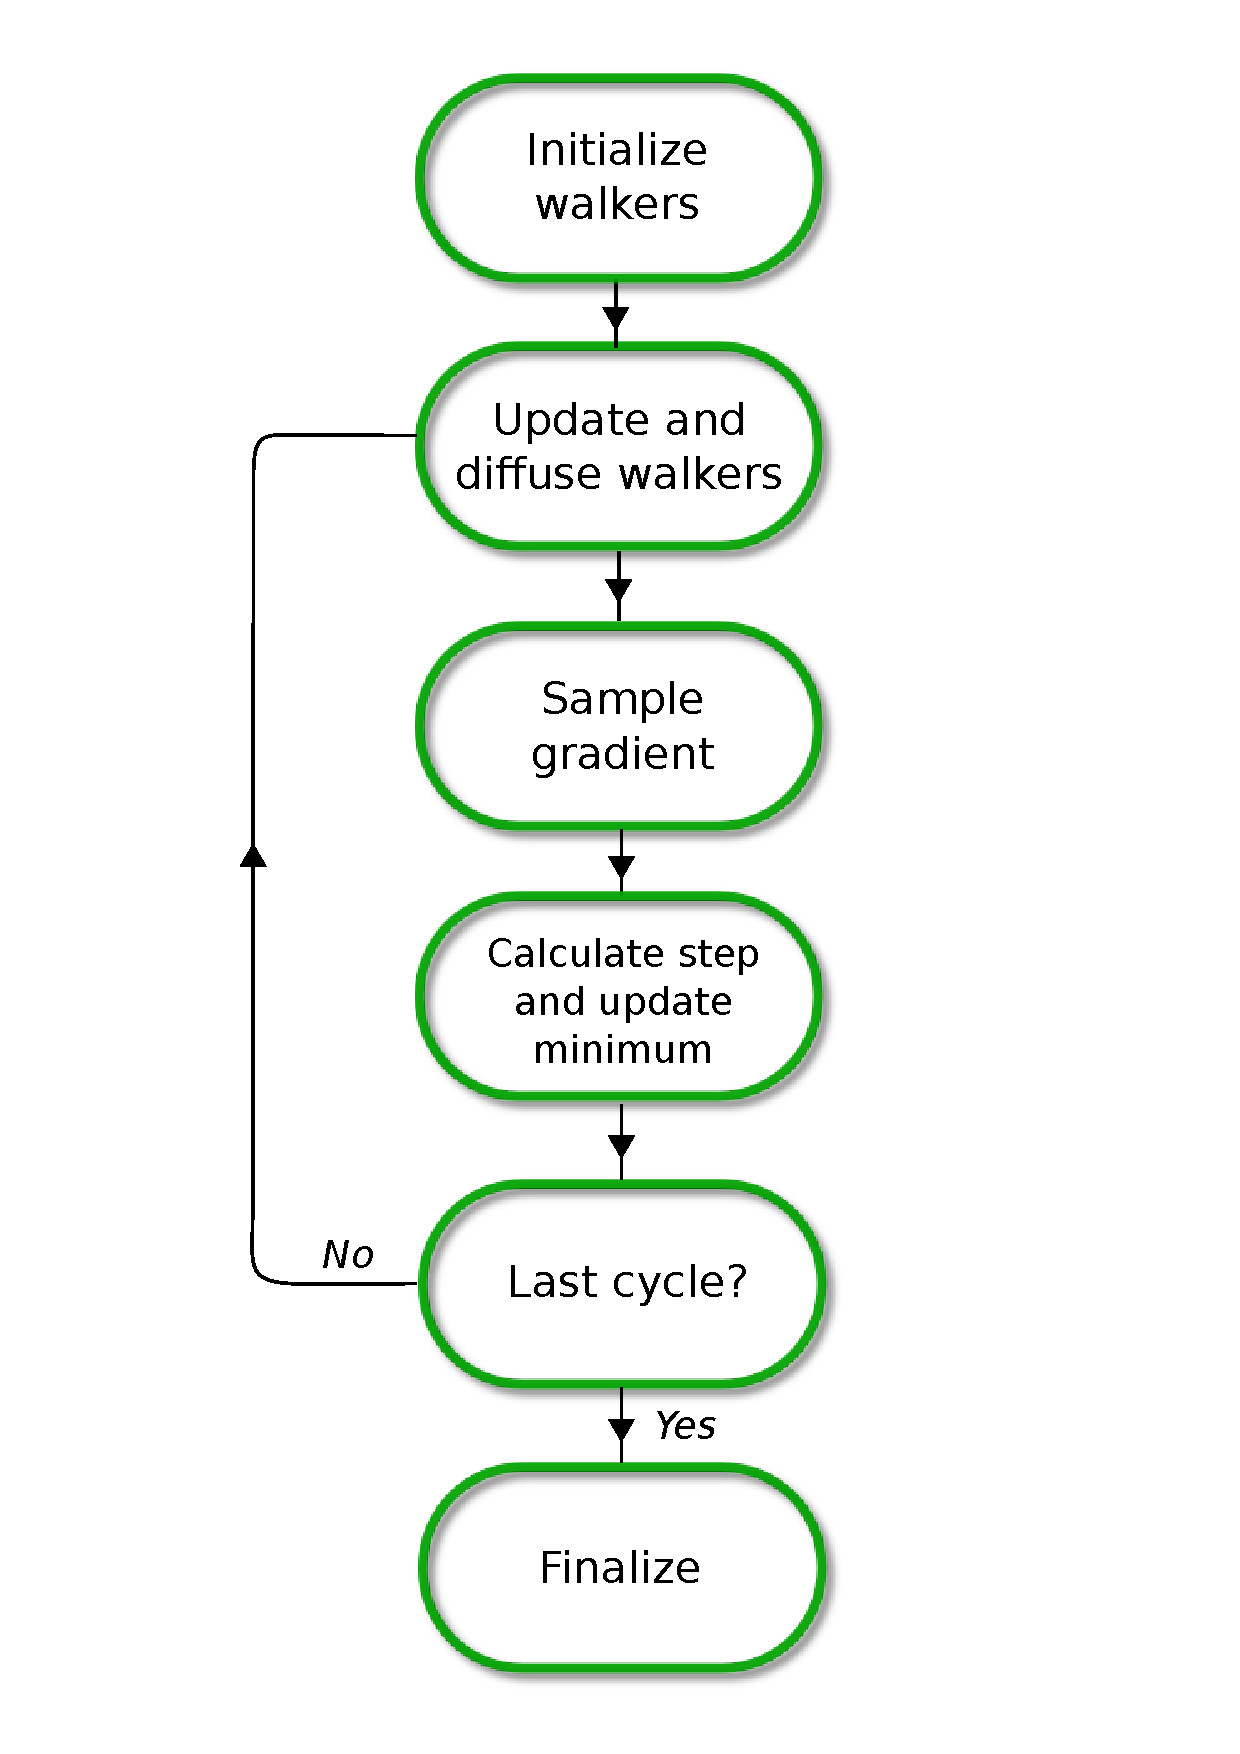
\includegraphics[scale=0.65]{../Graphics/ASGD_UML.pdf}
  \caption{Chart flow of ASGD algorithm. Diffusing a walker is done as described in Fig. \ref{fig:diffFlowChart}. Updating the walkers involves recalculating any values afflicted by updating the minimum. The step is calculated by Eq.~(\ref{eq:ASGD_delta_i}). In case of Quantum Monte-Carlo, the gradient is sampled by Eq.~(\ref{eq:varParGrad}).}
 \end{center}
\end{figure}
\clearpage


\section{Variational Monte-Carlo}
\label{sec:VMC}

Once a given 

\begin{figure}
\label{fig:VMCchart}
 \begin{center}
  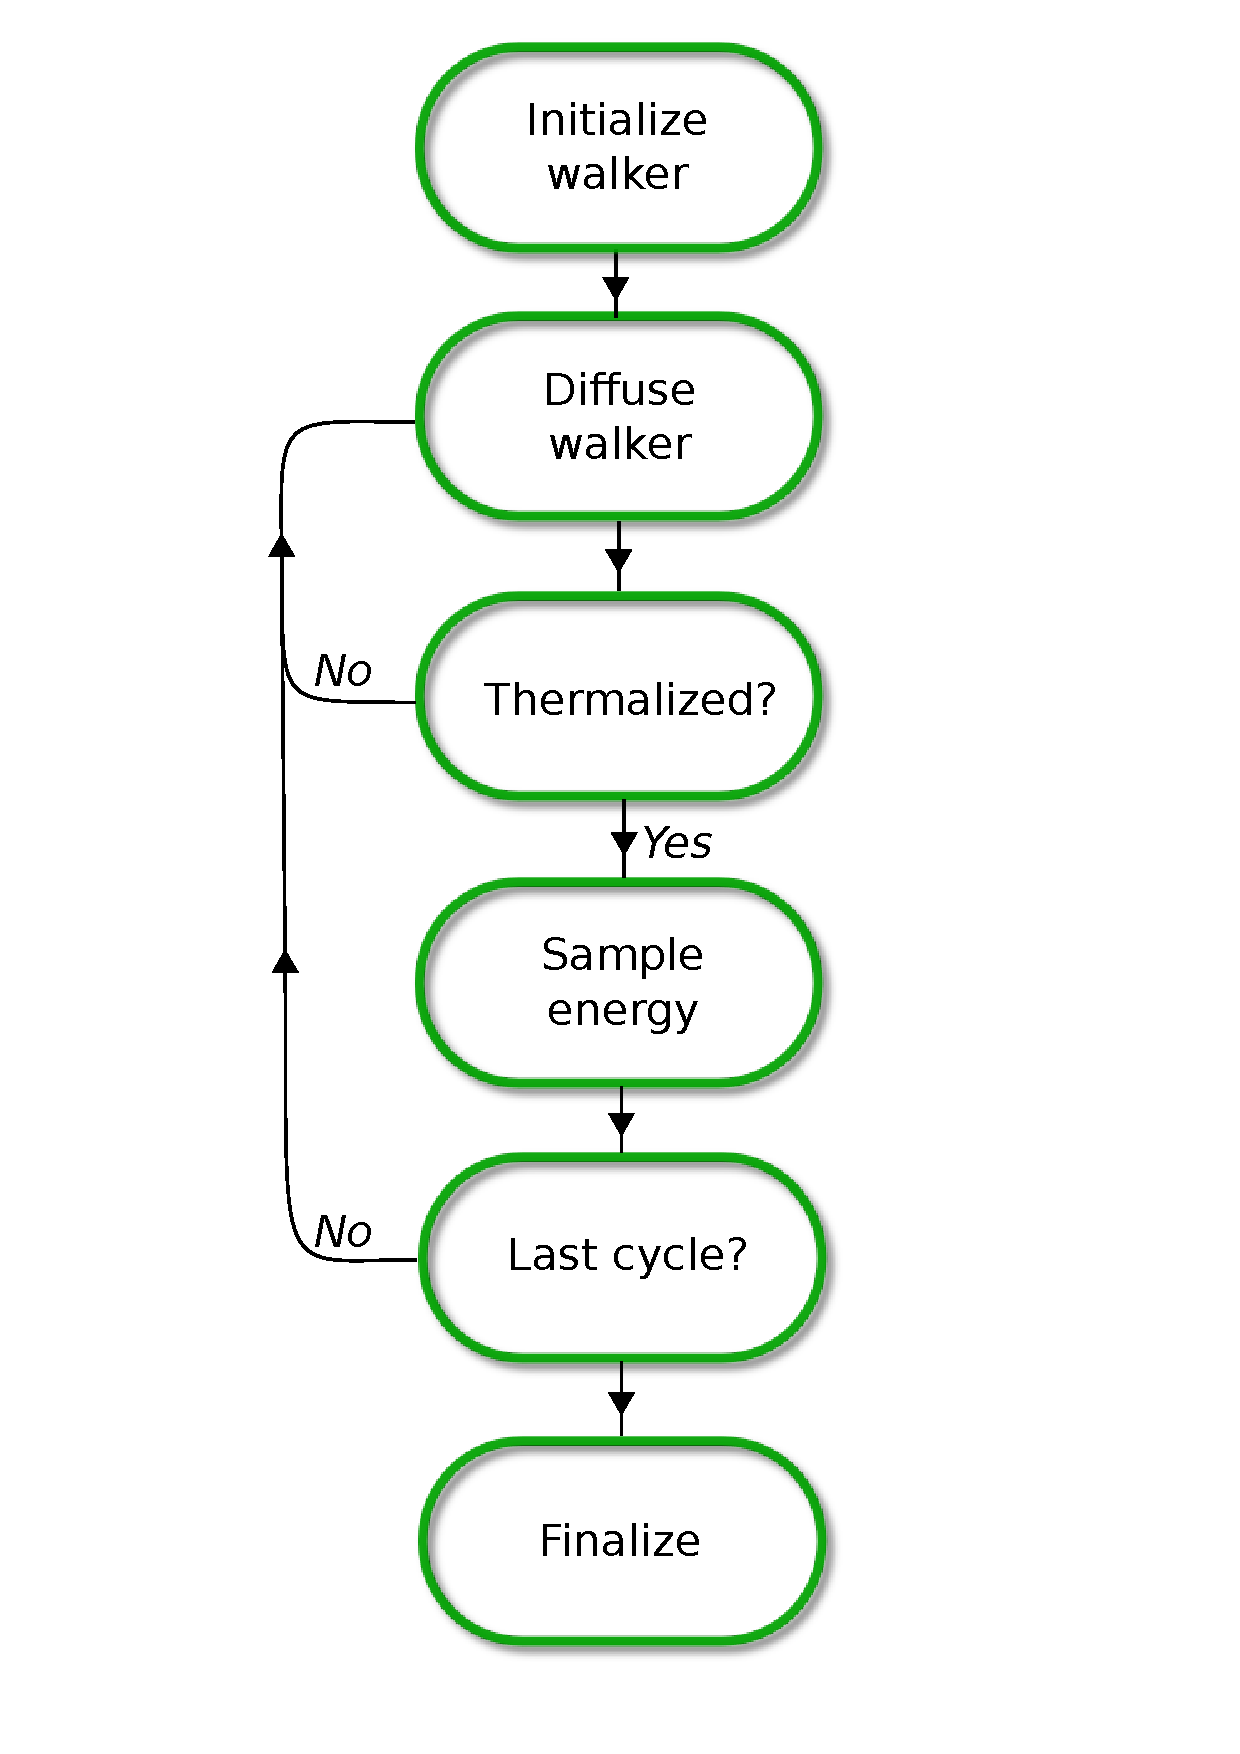
\includegraphics[scale=0.65]{../Graphics/VMCUML.pdf}
  \caption{Chart flow of the Variational Monte-Carlo algorithm. The second step, \textit{Diffuse Walker}, is the process described in Fig. \ref{fig:diffFlowChart}. Energies are sampled as described in Section \ref{sec:calcExpVals}. Thermalization is usually set to a fixed number of cycles. }
 \end{center}
\end{figure}
\clearpage

\section{Diffusion Monte-Carlo}
\label{sec:DMC}

\begin{figure}
\label{fig:DMCchart}
 \begin{center}
  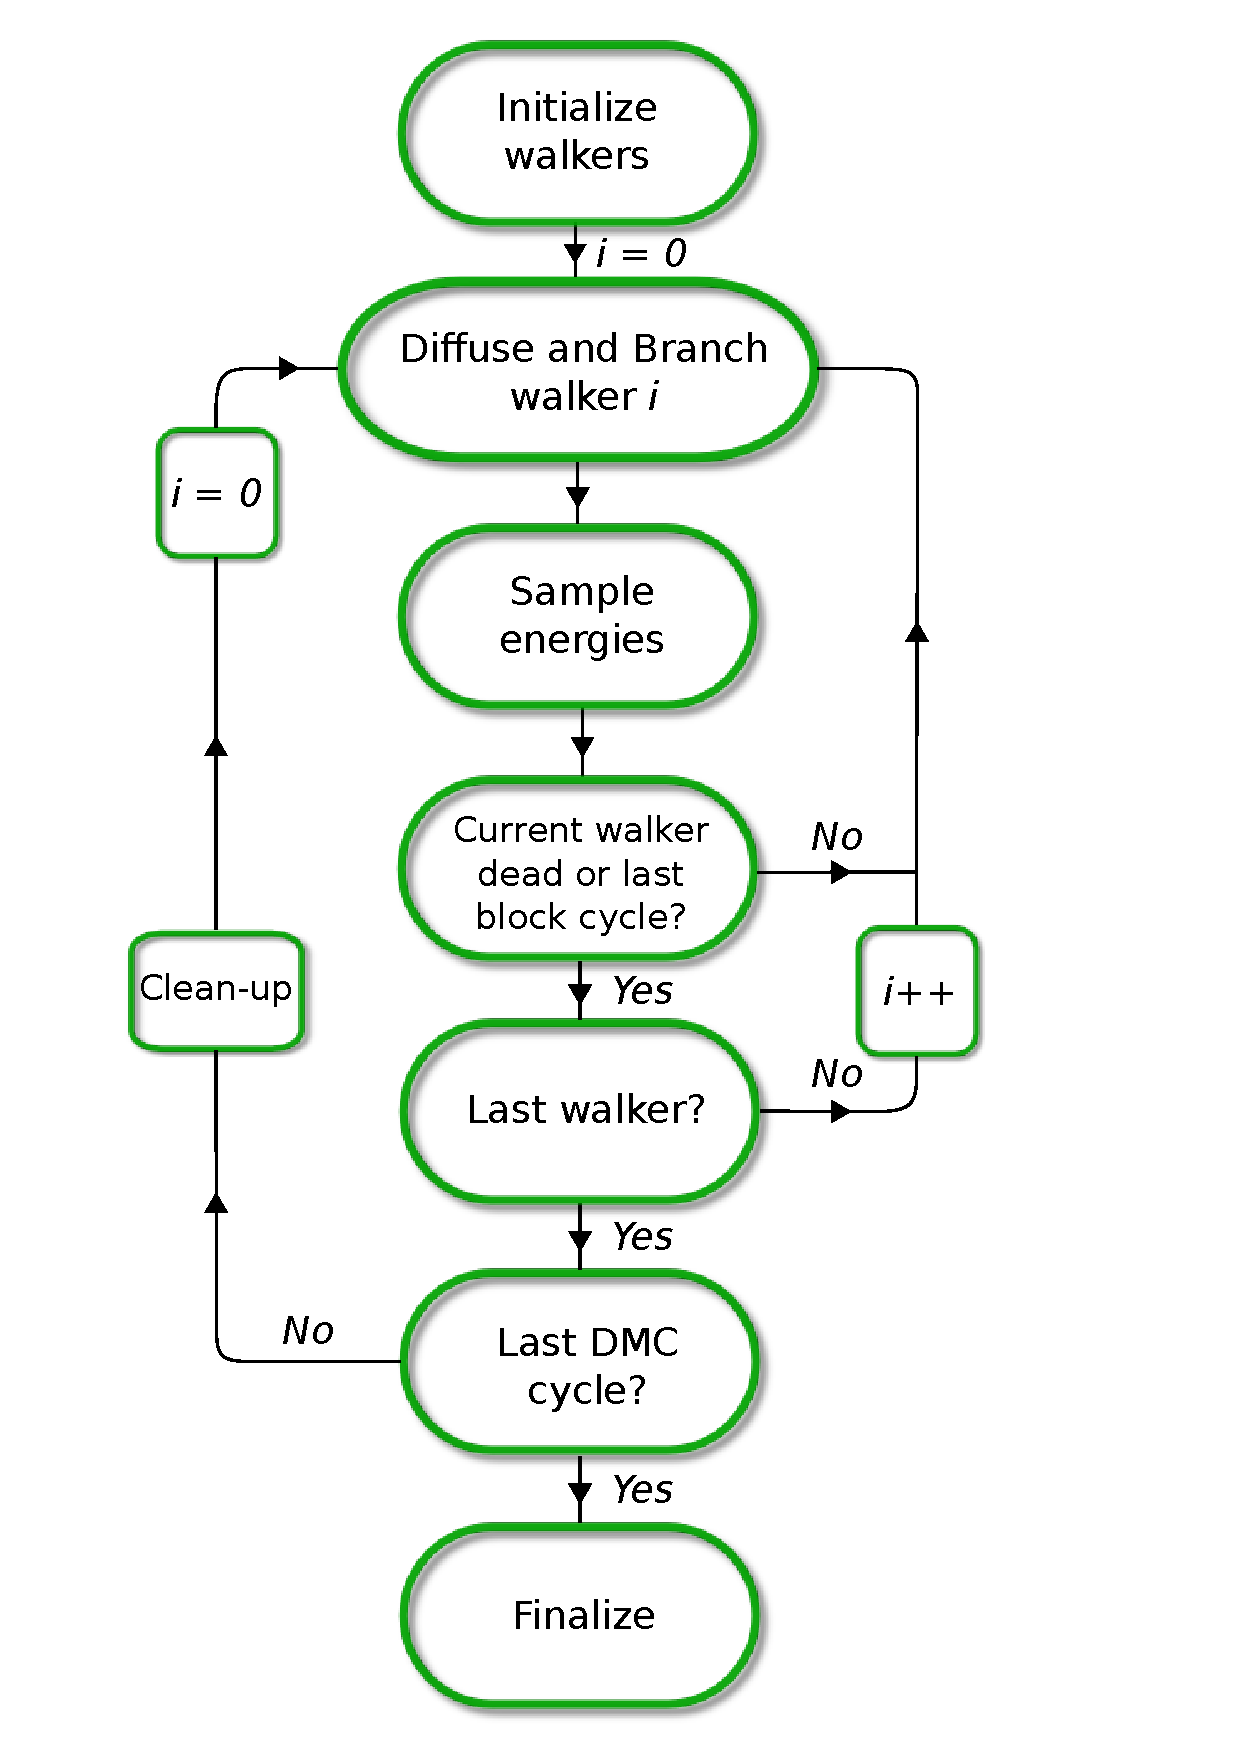
\includegraphics[scale=0.65]{../Graphics/DMCUML.pdf}
  \caption{Chart flow of the Diffusion Monte-Carlo algorithm. The count variable \textit{i} is the index of the walker loop. The second step, \textit{Diffuse and Branch Walker}, is the process described in Fig. \ref{fig:diffFlowChart} in combination with the branching from Fig. \ref{fig:branching}. Energies are sampled as described in Section \ref{sec:DMC}. Thermalization is not done in the same way as VMC (see Fig. \ref{fig:VMCchart}), but rather includes the entire flow with a reduced number of DMC - and block cycles. }
 \end{center}
\end{figure}
\clearpage

\section{Fixed node approximation}

Looking at Eq.~(\ref{eq:BosonicWFExplicit}), we notice that by choosing positive phases for our single particle wave functions, the bosonic many body wave function is exclusively positive. For fermions however, the sign change upon permuting a particle pair introduces the possibility that the wave function will have both negative and positive regions, independent of our choice of phases in the single particle wave functions.

As we simulate importance sampled DMC in time, the density of walkers at a given time, $P(x, \tau)$, is given by Eq.~(\ref{eq:schrodGeneralSolution2}) multiplied by the trial wave function (see the end of Section \ref{sec:anisFokker} for details)

\begin{equation}
 P(x, \tau) = \Phi(x, \tau)\Psi_T(x),
\end{equation}

where

\begin{equation}
  \lim_{\tau\to\infty} P(x, \tau) = \Phi_0(x)\Psi_T(x),
\end{equation}

which, if interpreted as a density, should always be greater than zero. In the case of Fermions, this is not guaranteed, as
the node structure, i.e. the roots, of the exact ground state and the trial wave function will generally be different.  

To avoid this anomaly in the density, $\Phi(x, \tau)$ and $\Psi_T(x)$ have to change sign together\footnote{It should be mentioned that more sophisticated methods exist for dealing with the sign problem, some of which splits the distribution of walkers into a negative and a positive region.}. The brute force way of solving this problem is to \textit{fix} the nodes by rejecting a walker's step if the trial wave function changes sign:

\begin{equation}
\frac{\Psi_T(x_i)}{\Psi_T(x_j)} < 0 \quad\Longrightarrow\quad A(i\,\rightarrow\,j) = 0
\end{equation}

where $A(i\,\rightarrow\,j)$ is the probability of accepting the move, as described in Section \ref{sec:MetroMain}. An illustrative example is attempted in Fig. \ref{fig:fixxednode}.

\begin{figure}
\label{fig:fixxednode}
 \begin{center}
  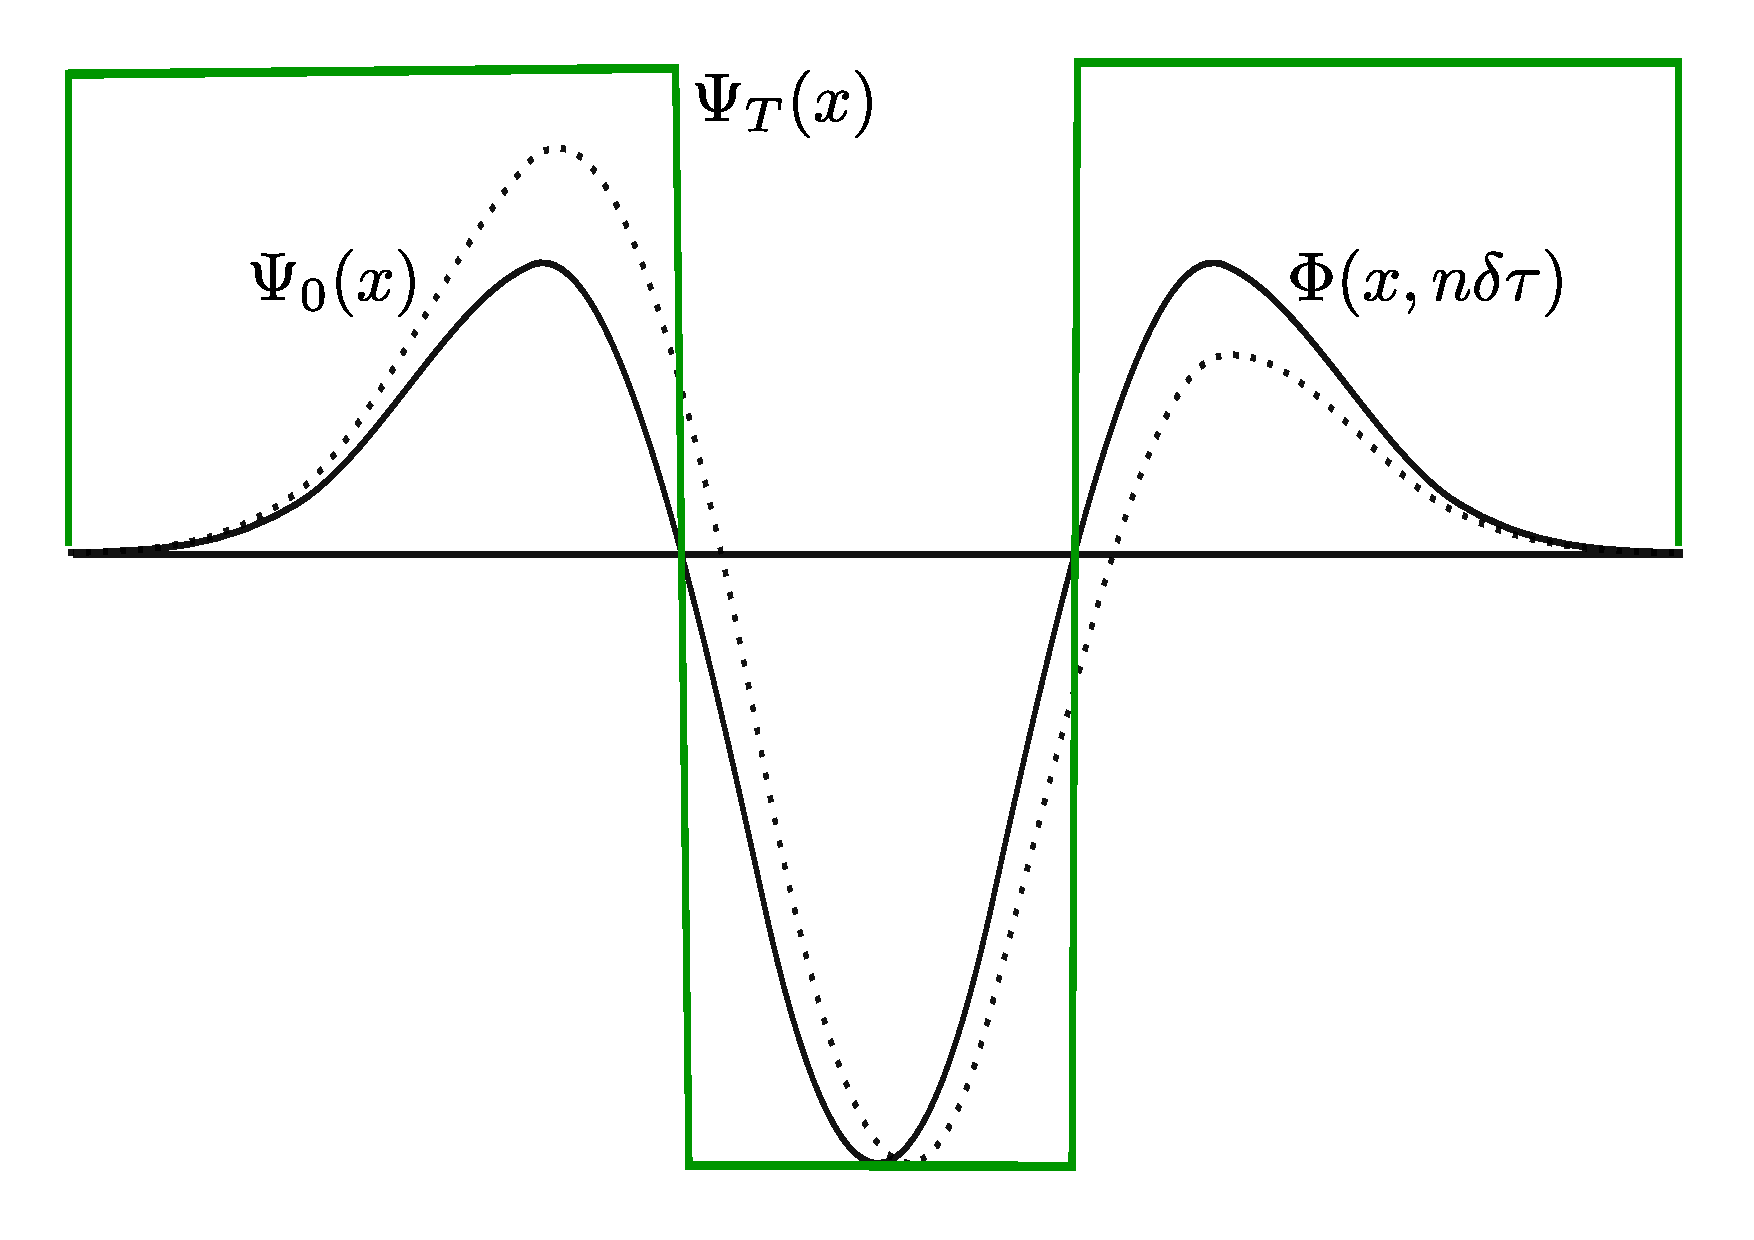
\includegraphics[scale=0.3]{../Graphics/fixxednode.pdf}
  \caption{An illustration of the fixed node approximation. The dotted line is the exact ground state $\Psi_0(x)$. The distribution of walkers at cycle $n$, $\Phi(x, n\delta\tau)$, similar in shape with $\Psi_0(x)$, however, sharing nodes with the trial wave function $\Psi_T(x)$ (box-like function for illustration purposes), and thus making it impossible to match the true ground state exactly.}
 \end{center}
\end{figure}



\section{Estimating the Statistical Error}

As with any statistical result, appropriate statistical errors needs to be included for it to be taken seriously. Systematic errors, that is, errors introduced due to limitations in the model, will be discussed in each method's respective section. Statistical errors, that is, the  deviation from the true ensemble average due to the fact that we can never fulfill the equality in Eq.~(\ref{eq:MeanVStrueExp}), can be estimated using several methods, some of which are \textit{naive} in the sense that they assume the dataset to be completely \textit{uncorrelated}. 

\subsection{The Variance and Standard Deviates}

Given a set of samplings, e.g. local energies, the variance is a measure of their spread from the true mean value

\begin{eqnarray}
\label{eq:variance}
\Var(E) &=& \Exp{(E-\Exp{E})^2} \nonumber\\
        &=& \Exp{E^2} - 2\underbrace{\Exp{E\Exp{E}}}_{\Exp{E}\Exp{E}} + \Exp{E}^2 \nonumber\\
        &=& \Exp{E^2} - \Exp{E}^2 \\
        &\simeq& \overline{E^2} - \overline{E}^2
\end{eqnarray}

In the case of having the exact wave function, i.e $\ket{\Psi_T} = \ket{\Psi_0}$, the variance becomes zero:

\begin{eqnarray*}
\label{eq:varianceZeroExact}
\Var(E)_\mathrm{Exact} &=& \bra{\Psi_0}\OP{H}^2\ket{\Psi_0} -  \bra{\Psi_0}\OP{H}\ket{\Psi_0}^2 \\
		        &=& E_0^2 - (E_0)^2 \\
		        &=& 0
\end{eqnarray*}

The variance is in other words an excellent measure of how good a fit different trial wave functions are to the system. Note however, a common misconception is to use the numerical value of the variance to compare \textit{different} systems; for instance, if system $A$ has variance equal to half of system $B$'s, one could easily conclude that system $A$ has the best fit. This is not true. The variance has units (in the case of local energies) energy squared, and will thus scale with the magnitude of the energy. One can only safely use the variance as a direct measure locally in each specific system, e.g. Beryllium simulations.

Another misconception is that the variance is a direct numerical measure of the error. This can in no way be true given that the units mismatch. The \textit{standard deviation}, $\sigma$, is the square root of the variance,

\begin{equation}
\label{eq:stdNaive}
 \sigma^2(x) = \Var(x),
\end{equation}


and has hence a unit equal to that of the measured value. It is therefore related to the \textit{spread} in the sampled value; zero deviation implies perfect samples, while increasing deviation means increasing spread and statistical uncertainty. The standard deviation is in other words a useful quantity when it comes to calculating the error, i.e. the expected deviation from the exact mean $\Exp{E}$.

\subsection{The Covariance and correlated samples}

It was briefly mentioned in the introduction that certain error estimation techniques was too naive in case of correlated samples. Two samples, $x$, $y$, are said to be correlated if their \textit{covariance}, $\Cov(x, y)$, is non-zero

\begin{eqnarray}
\label{eq:covariance}
 \Cov(x, y) &\equiv& \Exp{(x - \Exp{x})(y - \Exp{y})} \nonumber\\
            &=& \Exp{xy - x\Exp{y} - \Exp{x}y + \Exp{x}\Exp{y}} \nonumber\\
            &=& \Exp{xy} - \Exp{x\Exp{y}} \underbrace{-\Exp{y\Exp{x}} + \Exp{\Exp{x}\Exp{y}}}_{0} \nonumber\\
            &=& \Exp{xy} - \Exp{x}\Exp{y}.
\end{eqnarray}

Notice that $\Cov(x,x) = \Var(x)$. Using this definition, whether of not we have correlated samples boils down to whether or not $\Exp{xy} = \Exp{x}\Exp{y}$. 

The consequence of ignoring correlations is an error estimate which is generally less than the true error; correlated samplings are more clustered, i.e. less spread, due to previous samplings' influence on the value of the current sample. Denoting the true standard deviation as $\sigma_c$, the above discussion can be distilled to

\begin{equation}
 \label{eq:trueVsNaiveSTD}
 \sigma_c(x) \ge \sigma(x),
\end{equation}

where $\sigma$ is the deviation from Eq.~(\ref{eq:stdNaive}). 


\subsection{The Deviate from the Exact Mean}

There is an important difference between the deviate from the exact mean, and the deviate of a single sample from it's combined mean, i.e.

\begin{equation}
 \sigma(\overline{x}) \ne \sigma(x).
\end{equation}

Imagine doing a number of simulations, each resulting in a unique $\overline{x}$, the quantity of interest is not the deviation within a single simulation, but the deviation between all the simulations.

\begin{eqnarray}
 m &\equiv& \overline{x} = \frac{1}{n}\sum_{i=1}^n x_i \label{eq:meanx}\\
 \sigma^2(m) &=& \Exp{m^2} - \Exp{m}^2 \label{eq:sigma_m}
\end{eqnarray}

Combining the above equations yields

\begin{eqnarray}
\label{eq:realErrorCovariance1}
  \sigma^2(m) &=& \Exp{\frac{1}{n^2}\left[\sum_{i=1}^nx_i\right]^2} - \Exp{\frac{1}{n}\sum_{i=1}^n x_i}^2 \nonumber\\
              &=& \frac{1}{n^2}\left( \Exp{\sum_{i=1}^n x_i\sum_{j=1}^n x_j} - \Exp{\sum_{i=1}^n x_i}\Exp{\sum_{j=1}^n x_j}  \right) \nonumber\\
              &=& \frac{1}{n^2}\sum_{i,j=1}^n \Exp{x_ix_j} - \Exp{x_i}\Exp{x_j} \nonumber\\
              &=& \frac{1}{n^2}\sum_{i,j=1}^n \Cov(x_i, x_j)
\end{eqnarray}

This result is important; the true error is given in terms of the covariance, and is, as discussed previously, only equal to the sample variance if our samples are uncorrelated. Going back to the definition of covariance in Eq.~(\ref{eq:covariance}), we see that in order to calculate the covariance as in Eq.~(\ref{eq:realErrorCovariance1}), we need to know the true mean $\Exp{x_i}$. Using $m=\overline{x}$ as an approximation to the true mean yields   

\begin{eqnarray}
 \Cov(x_i, x_j) &\equiv& \Exp{(x_i - \Exp{x_i})(x_j - \Exp{x_j})} \nonumber\\
                &\simeq& \Exp{(x_i - m)(x_j - m)} \nonumber\\
                &\simeq& \frac{1}{n^2}\sum_{k,l=1}^n (x_k-m)(x_l-m) \\
                &\equiv& \frac{1}{n}\Cov(x)
\end{eqnarray}

Inserting this relation into Eq.~(\ref{eq:realErrorCovariance1}) yields

\begin{eqnarray}
\label{eq:realErrorCovariance2}
   \sigma^2(m) &=& \frac{1}{n^2}\sum_{i,j=1}^n \Cov(x_i, x_j) \nonumber\\
               &\simeq& \frac{1}{n^2}\sum_{i,j=1}^n \frac{1}{n}\Cov(x) \nonumber\\
               &=& \frac{1}{n^3}\Cov(x)\underbrace{\sum_{i,j=1}^n}_{n^2}  \nonumber\\
               &=& \frac{1}{n} \Cov(x),
\end{eqnarray}

which serves as a practical way of calculating the full error (including correlations). 

Explicitly computing the covariance is rarely done in Monte-Carlo simulations; if the sample size is large, it is extremely expensive. A variety of alternative methods to counter the correlations are available, the simplest of which is to define a \textit{correlation length}, $\tau$\footnote{This parameter is often referred to as the \textit{auto-correlation time} in the literature.}, which defines an interval at which points from the sampling sets are used for actual averaging. In other words, only the points $x_0, x_{\tau}, ..., x_{n\tau}$ are used in the calculation of $\overline{x}$

\begin{equation}
 \overline{x} = \frac{1}{n}\sum_{k=0}^n x_{k\cdot\tau}
\end{equation}

This basically means that we need $n\tau$ samples in order to get the same magnitude of samples to our average as in Eq.~(\ref{eq:meanx}); the \textit{effective sample size} becomes $n_\mathrm{eff} = n_\mathrm{tot}/\tau$. $\tau = 1$ defines the uncorrelated case. For details regarding the derivations of $\tau$ based on the covariance, see ref. \cite{flyvbjerg:461} and ref. \cite{morten}.

\subsection{Blocking}

Introducing correlation lengths in the system solver is not an efficient option. Neither is calculating the covariance of billions of data points. However, the error is not a value vital to the simulation process, i.e. you do not need to know the error at any stage during the sampling. This means that we can post process the error calculation (given that we store the data sets).

An efficient algorithm for calculating the error of correlated data is \textit{blocking}. This method is described in high detail in ref. \cite{flyvbjerg:461}, however, details aside, the idea itself is quite intuitive: Given a data set of $N$ samples from a single Monte-Carlo simulation, imagine dividing the dataset into \textit{blocks} of $n$ samples, that is, blocks of size  $n_b=N/n$. The error $\sigma_n$ in each block will increase as $n$ decrease, (see Eq.~(\ref{eq:realErrorCovariance2}))

\begin{equation}
 \sigma_n \propto \frac{1}{\sqrt{n}}
\end{equation}


However, treating each block as an individual simulation, we have $n_b$ averages $m_n$ that we can use to calculate the total error in Eq.~(\ref{eq:sigma_m}), that is, estimate the covariance

\begin{eqnarray}
  \overline{m_n^r} &\equiv& \frac{1}{n_b}\sum_{k=1}^{n_b} m_n^r \\
\nonumber\\
  \sigma^2(m) &=& \Exp{m^2} - \Exp{m}^2 \nonumber\\
              &\simeq& \overline{m_n^2} - (\overline{m_n})^2 \label{eq:blockingError}
\end{eqnarray}

The approximation should hold for a range of different block sizes, however, just as there is no a priori way of telling the correlation length, there is no a priori way of telling how many blocks is needed. What we do know however, is that if the system is correlated, there should be a range of different block sizes which fulfill Eq.~(\ref{eq:blockingError}) to reasonable precision. The result of a blocking analysis is therefore a series of ($n$, $\sigma(m)$) pairs. Plotting these pairs should in light of previous arguments result in a increasing curve which stabilizes over a certain span of block sizes. This plateau will then serve as a reasonable approximation to the covariance. See Fig. \ref{FIG:BlockingExamples} for a demonstration of the blocking technique.

\begin{figure}
\label{FIG:BlockingExamples}
 \begin{center}
  \subfigure{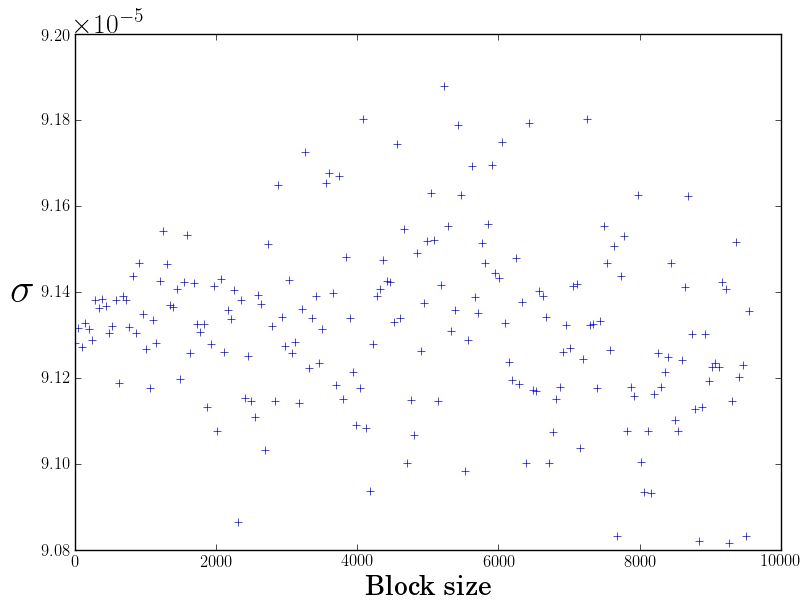
\includegraphics[scale=0.35]{../Graphics/BlockingExampleUncorr.png}}
  \subfigure{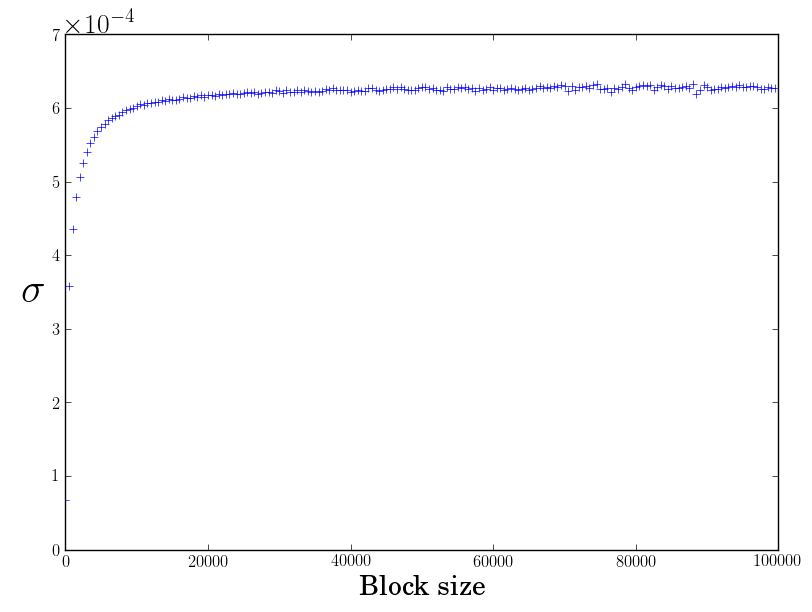
\includegraphics[scale=0.35]{../Graphics/BlockingExampleCorr.png}} 
  \caption{Left hand side: Blocking result of (approximately) uncorrelated data generated from a uniform Monte-Carlo integration of $\int _1^2 2x\mathrm{d}x$ resulting in $3.00003$ (exact is $3.0$). This is in excellent agreement with the magnitude of the error $\sim 9\cdot 10^{-5}$. On the right hand side we have the blocking result (DMC) for 6-particle $\omega=0.1$ Quantum Dot, used in Table \ref{tab:QDotsResultsAll}. We clearly see the plateau discussed in the blocking section, resulting in a total error in the range of $4.5\cdot 10^{-5}$ to $5\cdot 10^{-5}$.}
 \end{center}
\end{figure}


\subsection{Variance Estimators}

The standard intuitive variance estimator given by

\begin{equation}
\label{eq:varBias}
 \sigma^2(x) \simeq \frac{1}{n}\sum_{i=1}^n (x_i - \overline{x})^2 = \left(\frac{1}{n}\sum_{i=1}^n x_i^2\right) - \overline{x}^2
\end{equation}

is just an example of a variance estimator. A more precise estimator is 

\begin{equation}
\label{eq:varUnbias}
 \sigma^2(x) \simeq \frac{1}{n-1}\sum_{i=1}^n (x_i - \overline{x})^2 = \left(\frac{1}{n-1}\sum_{i=1}^n x_i^2\right) - \frac{n}{n-1}\overline{x}^2
\end{equation}

which is only noticeably different from Eq.~(\ref{eq:varBias}) when the sample size gets small, as in blocking analysis. It is therefore standard to use Eq.~(\ref{eq:varUnbias}) for blocking errors.


